\chapter{Method}

%\section{Introduction}
%write what this chapter coveres. you have to bring relation to chapter 2 here.
This chapter will describe different methodologies used to solve technical problems over the course of this project.

\section{Problem Formulation} \label{sec:M:ProblemFormulation}
As described in section \ref{sec:I:Objective}, the objective of this project is to modify the existing mobile robot from the report in appendix \ref{A:MAS513Report} so that it is capable of preforming a warehouse automation task. The solution should be tested in a scenario where the robot is tasked with fetching and object from a given location, and delivering this object to a predefined location. The following list will provide a better understanding of the test scenario and the order in which the different tasks should be preformed.

\begin{enumerate}
    \item Autonomously navigate to a given "pick pose".
    \item Search for the defined object using machine vision.
    \item Pick the defined object using a manipulator mounted on the mobile robot.
    \item Autonomously navigate to a predefined "place pose".
    \item Place the object on the place location.
    \item Autonomously navigate back to the starting point.
\end{enumerate}




% aj try to use the termology and functionalities in ch. 2 and show how they can be used to achieve your goal. Explain well write entire sequency from navigation, collission detection and avoidance, object localization using tag, pick from a given co-ordinate and place at other.

%aj \section{Material and Method} 3.3
%aj a block diagram explaining how the building blocks in chapter 2 is connected plus the tools e.g. HW, SW, ROS network ..., then explain each block in different section. 
% 3.3.1 autonomous navigation. Explain the block diagram that does navigation, collission detection and avoidance with algorithm e.g. SLAM how it is done (NAV2) ory you can directly say you used NAV2 [] for this
% 3.3.2 Object localization and pose estimation. Explain with block diagram and algorithm, flowchart
% 3.3.4 Pick and place. How this is done. Write block diagram, flowchart and algorithm.
        %3.3.1-3.3.4 is basically 3.5+3.6
% 3.3.5 coordinated action. Explain about master controller that decides the action in sequence 3.1-3. This is basically 3.6.3
%3.3.6 Experimental setup or UGV platform development - combine 3.2+3.3+3.4. Instead of different section, write in a paragraphs (one paragraph for each functionality) in contnuous fashion.


\section{Conceptual Design}\label{sec:M:ConceptualDesign}
The warehouse automation scenario described in section \ref{sec:M:ProblemFormulation}, can be divided into three main parts; an autonomous navigation system, a pick and place system, and the top level system that fuses "autonomous navigation" and "pick and place" together. Figure \ref{fig:M:CD:topLevelMethod} illustrates on a high level how these systems interact.

\begin{figure}[htp]
    \centering
    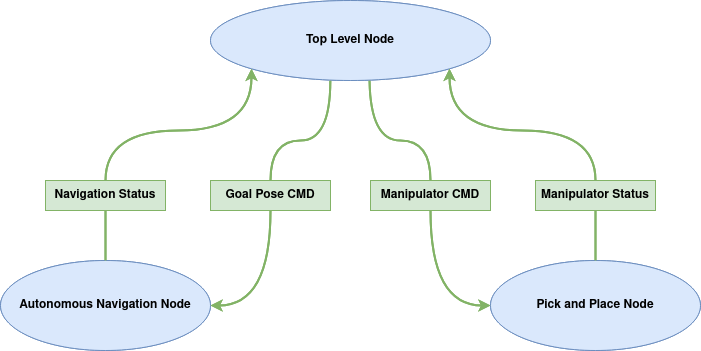
\includegraphics[width = 0.9\textwidth]{Figures/figTopLevelMethod.drawio.png}
    \caption{This figure illustrates on a high level how the main systems in the solution interacts with each other to orchestrate a warehouse automation task. The "Top Level" system sends commands and receives feedback from the two other systems "Autonomous Navigation" and "Pick and Place"}
    \label{fig:M:CD:topLevelMethod}
\end{figure}

The top level system should take commands for what object to pick and where this object is located in the warehouse. It should then give commands to both the autonomous navigation system and the pick and place system in order to orchestrate the defined warehouse automation scenario described in the problem formulation, sec \ref{sec:M:ProblemFormulation}. During this operation, this system will need some information on the status of the other systems to be able to orchestrate the scenario correctly.

The autonomous navigation system should be able to take goal poses consisting of $x,y,\theta$ coordinates, from the top level system. It should then plan it's trajectory, using either Djikstra's algorithm or A*, and autonomously navigate towards the goal pose without the assistance of any operator. During this operation, a SLAM algorithm should be running to provide an updated map of the robot's environment as well as robust localisation. It should also have a collision avoidance system capable of detecting and avoiding collision with moving objects such as workers in the warehouse. When the mobile robot has reached it's goal, the system should report back to the top level system that the goal has been reached. This is already set up during the course MAS-513-G, however, modifications have been done to accommodate the additions of other systems.

The pick and place system should consist of a manipulator and a machine vision system that will be a part of the mobile robot. The system should be able to take commands from the top level system and act accordingly. Example of commands are "pick", "place" and "sleep". During picking, machine vision should be utilised for object detection and pose estimation. The system should give feedback on it's current status to the top level system.

\subsection{Choice of Components} \label{sec:M:CD:ChoiceOfComponents}
The design of the robot should reflect the intended warehouse automation task. This places some requirements on the design that needs to be considered when setting up the robotic system. Design considerations in terms of component choice, regards the pick and place system, as the components for the mobile robot are provided before this project. The provided components are listed below as:

\begin{itemize}
    \item Clearpath - Husky A200 UGV
    \item Ouster - OS1-64 3D LiDAR
    \item Redshift Labs - UM7 IMU
    \item 2 X NVIDIA - Jetson AGX Xavier
\end{itemize}

A design requirement for all components chosen in this project, is compatibility with Robot Operating System 2(ROS 2). This has also been a design requirement for the components chosen for the MAS-513-G project. ROS 2 is an open source software development kit (SDK) for developing robots. This system acts as a middleware that takes care of the communication between components \cite{https://doi.org/10.48550/arxiv.1711.06396}. ROS 2 also contains a large open source library of algorithms for common robotic applications like EKF, SLAM, manipulator planning, autonomous navigation to name a few. Additionally, it contains development tools for visualisation, simulation, debugging, and more \cite{https://doi.org/10.48550/arxiv.1711.06396}. Finally, it is important to mention that there are different ROS 2 distributions and this project mainly uses focuses around Galactic Geochelone.

It can be seen that there are two NVIDIA Jetson AGX Xaviers mounted on the UGV. One of these is intended to take care of the autonomous navigation system along with all it's sensors. The other one is free as it stands before project startup. Therefore, it becomes natural to run the pick and place system on this extra computer. The concept is therefore largely focused around the pick and place system. The main hardware considerations in this system regards choosing a robotic manipulator that is small enough to be mounted on the UGV along with deciding where to mount the vision sensor and what vision sensor should be used. 

Considering the given design criteria, the following components were chosen for the pick and place system:

\begin{itemize}
    \item Interbotix - VX300 5-DOF Manipulator
    \item Intel - Realsense D435i Camera
\end{itemize}

 The Interbotix VX300, seen in figure \ref{fig:M:CD:FC:VX300}, is a 5-DOF manipulator with a specified payload of $750[g]$ and a reach of $750[mm]$, as specified in table \ref{tab:M:CD:FC:VX300Specs}. For the vision system, it was decided to mount a Realsense camera to the gripper of the robot. The Intel Realsense D435i is a stereoscopic camera, for machine vision applications, capable of providing 3D information of the environment. This camera provides the information necessary to preform object detection and pose estimation with point cloud data, for example using "PointPoseNet" as described in section \ref{sec:T:MachineVision}. However, for this project, a fiducial tag based vision system, also described in section \ref{sec:T:MachineVision}, is chosen.

\begin{figure}[htp]
  \centering
  \begin{minipage}[b]{0.49\textwidth}
        \centering
        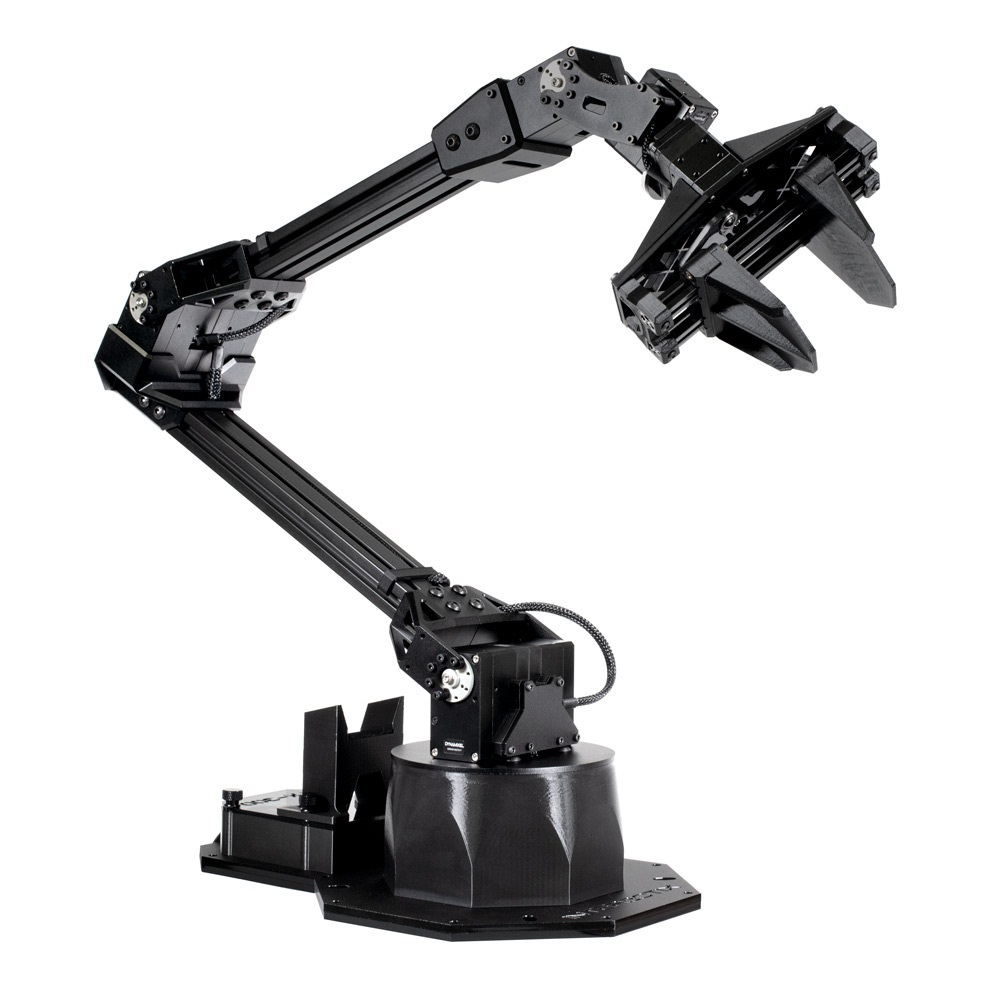
\includegraphics[width = 0.8\textwidth]{Figures/VX300.jpg}
        \caption{Interbotix VX300 5-DOF robotic manipulator. Image from \cite{interbotix_vx300}}
        \label{fig:M:CD:FC:VX300}
  \end{minipage}
  \hfill
  \begin{minipage}[b]{0.49\textwidth}
    \centering
    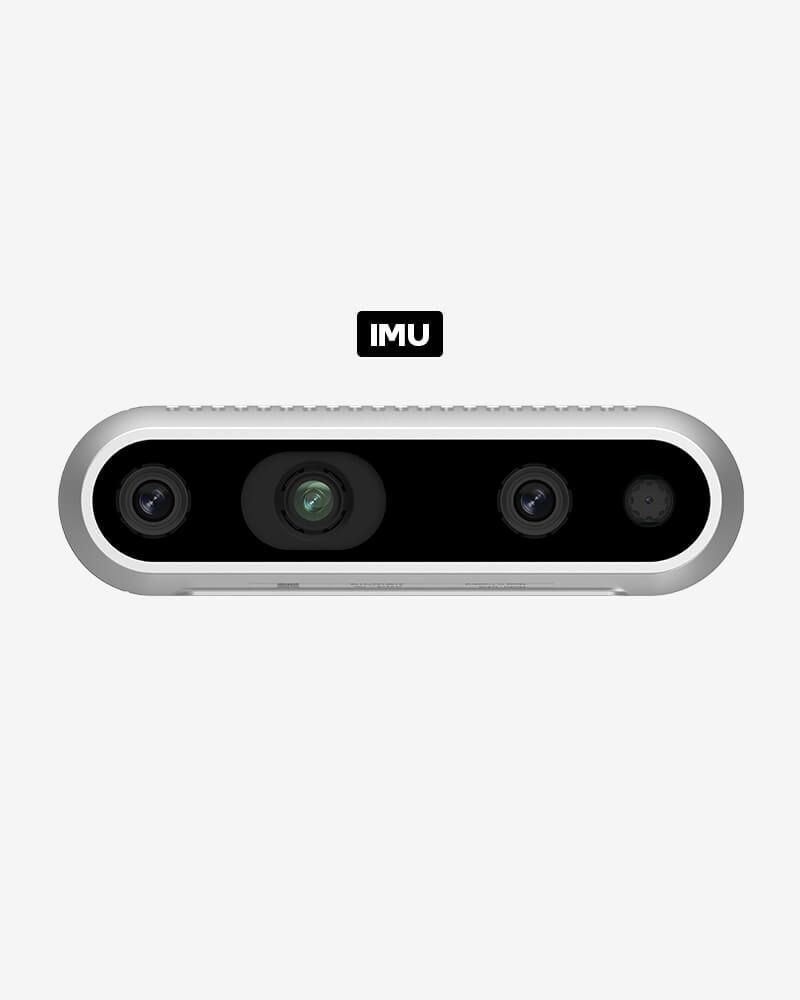
\includegraphics[width = 0.8\textwidth]{Figures/D435i.jpg}
    \caption{Intel Realsense D435i Stereoscopic Depth Camera. Image from: \cite{realsense_d435i}.}
    \label{fig:d435i}
  \end{minipage}
\end{figure}



% \begin{figure}[htp]
%   \centering
%   \begin{minipage}[b]{0.49\textwidth}
%         \centering
%         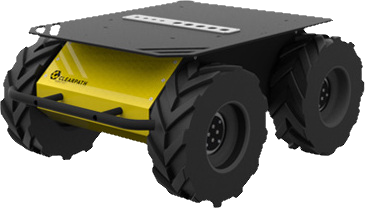
\includegraphics[width = 0.8\textwidth]{Figures/huskyA200.png}
%         \caption{Clearpath Husky A200. Image adapted from \cite{clearpath_husky_website}}
%         \label{fig:huskyA200}
%   \end{minipage}
%   \hfill
%   \begin{minipage}[b]{0.49\textwidth}
%     \centering
%     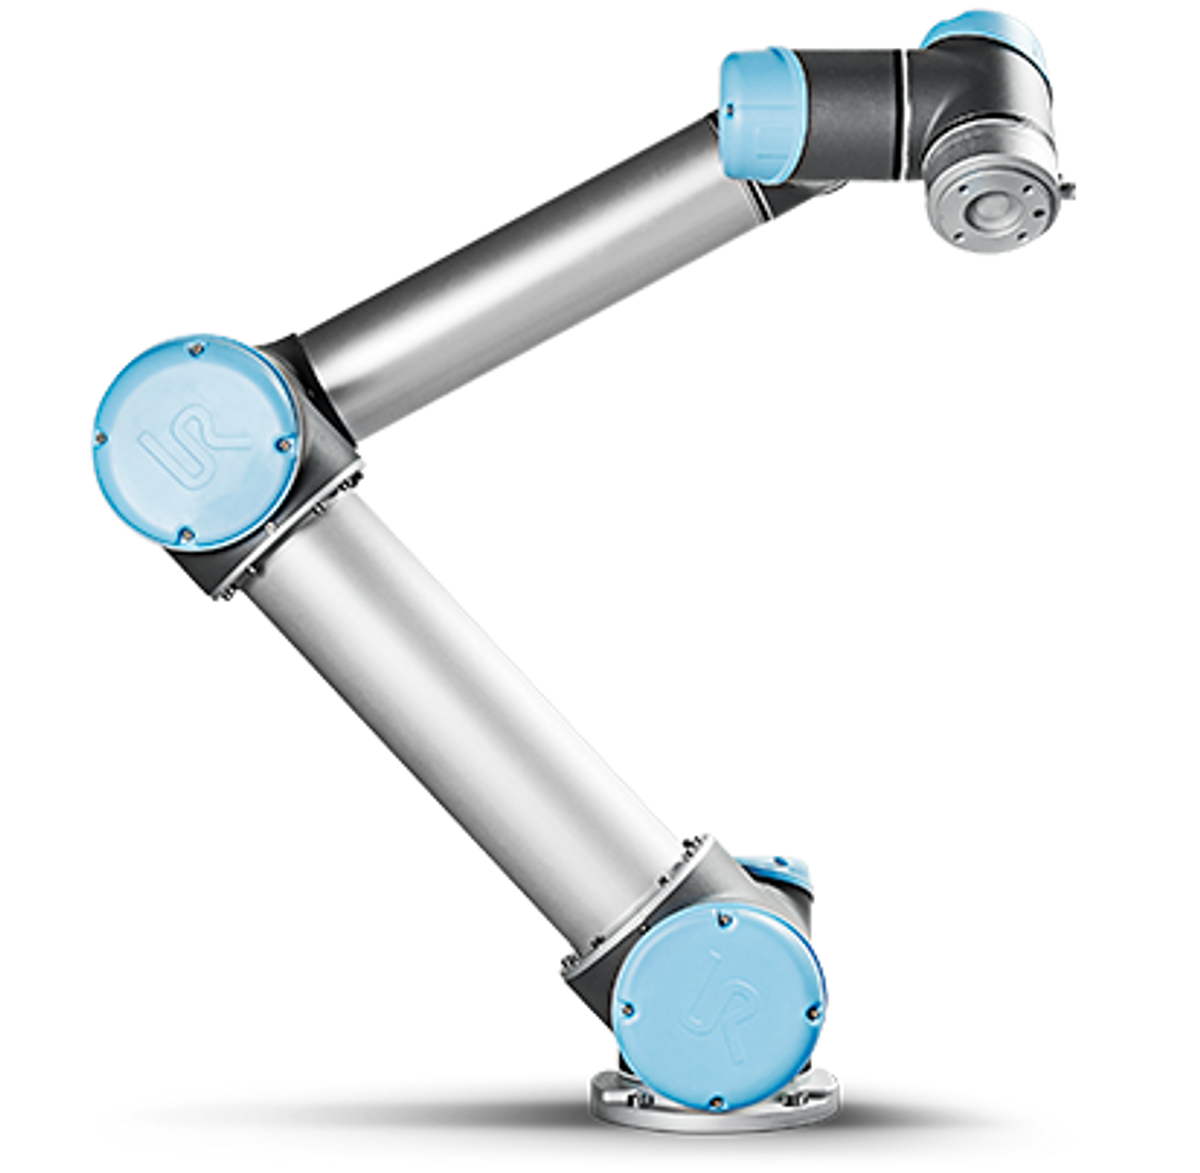
\includegraphics[width = 0.8\textwidth]{Figures/ur5.png}
%     \caption{Universal Robots UR5. Image from \cite{ur5_img}}
%     \label{fig:ur5}
%   \end{minipage}
% \end{figure}

% Some specifications on the Husky A200 robotic platform is listed in table \ref{tab:husky:a200:specs}

% \begin{table}[H]
\centering
\caption{Technical specifications for the Clearpath Husky A200, complete data sheet available in appendix \ref{A:fig:husky_data_sheet}, from \cite{clearpath_husky_website}}
\label{tab:husky:a200:specs}
\vspace{1mm}
\begin{tabular}{ll}
\hline
\multicolumn{2}{c}{\textbf{Husky A200 Specifications}}                                                            \\ \hline
Drivers and APIs                            & ROS, ROS 2, C++ and Python                                          \\
Wheel encoders                              & Quadrature: 78,000 {[}pulses/m{]}
        \\
Communication                               & RS232@115200 Baud                                                   \\
Battery                                     & \begin{tabular}[c]{@{}l@{}}12V 20Ah\\ Sealed Lead Acid\end{tabular} \\
\multicolumn{1}{c}{User Power Distribution} & \begin{tabular}[c]{@{}l@{}}5V 5A\\  12V 5A\\  24V 5A\end{tabular}   \\
Weight                                      & 50 {[}kg{]}                                                         \\
Payload Capacity                            & 75 {[}kg{]}                                                         \\
External Dimensions                         & 990 x 670 x 390 {[}mm{]}                                            \\ \hline
\end{tabular}
\end{table}

% One NVIDIA Jetson AGX Xavier, hereby called "UGV Xavier", interfaces with Husky, LiDAR and IMU. This computer will control the Husky and take care of autonomous navigation tasks such as mapping, localization and path planning. 

% The second NVIDIA Jetson AGX Xavier, hereby called Manipulator Xavier, interfaces with the Realsense camera and robotic manipulator. This computer will control the manipulator, and take care of sensory information from the Realsense camera. 

% The relatively powerful GPU of the Xaviers adds capabilities to implement deep learning algorithms to do for example image- or PointCloud based object detection.



  
\section{Hardware Architecture}\label{sec:M:Hardware}
This section describes the different hardware components of the robotic system and how they are set up for this project. A high level overview of the network topology is shown in figure \ref{fig:topology}. This topology gives an insight to how the different components are connected to create a complete system. Looking at figure \ref{fig:topology}, it can be seen that the UGV Xavier communicates with the Husky through RS232 and the UM7 IMU through USB. The LiDAR communicates through Ethernet via a WiFi router that, in this case acts as a switch. The LiDAR data is therefore available for all computers on the network. From figure \ref{fig:topology}, it can be seen that the Manipulator Xavier interfaces with both the Realsense camera and the manipulator through USB. 

\begin{figure}[htp]
  \centering
  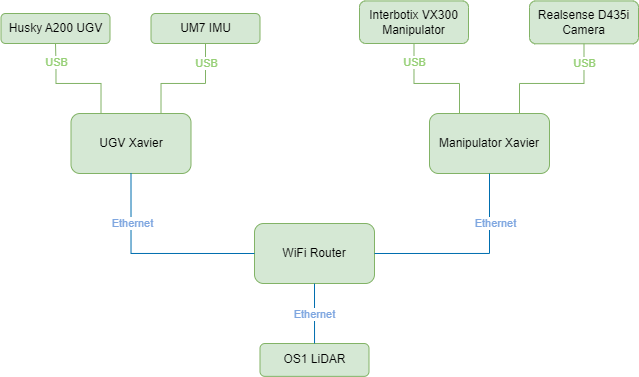
\includegraphics[width = 0.9\textwidth]{Figures/example_figure.drawio.png}
  \caption{High level network topology showing the various components on the mobile robotic platform}
  \label{fig:topology}
\end{figure}
%AJ your laptop that runs top level node is missing

The WiFi Router allows external computers to connect to the network, either through WiFi or cabled connection, and communicate with the two Xaviers and the LiDAR. This makes it possible to control the Xavier computers through SSH and also allows developers to interact with the ROS2 network.


\subsection{Auxiliary Hardware Components} \label{sec:M:HA:AuxiliaryHardware}
%\subsection{Accessory mounting frame}\label{sec:M:H:AccessoryMountingFrame}
As the UGV is to be used for prototyping and testing, it is preferable to have some kind of bracket where various sensors and actuators could be mounted. The bracket should be rigid, yet flexible in terms of mounting possibilities. An aluminium profile frame is therefore designed for the UGV. The aluminium frame, seen in figure \ref{fig:M:H:AMF:userFrame} is made out of 20X20mm aluminium profiles. The purpose of the frame is to add the possibility to mount whatever accessory the developer wants to the UGV. The choice fell on 20X20mm aluminium profiles as they are practical for mounting various equipment as well as the fact that the Husky A200 UGV is delivered with a 20x20mm mounting frame out of the box. Looking at figure \ref{fig:M:H:AMF:userFrame}, the husky mounting frame can be seen as the rectangular black frame on top of the Husky UGV.

\begin{figure}[htp]
  \centering
  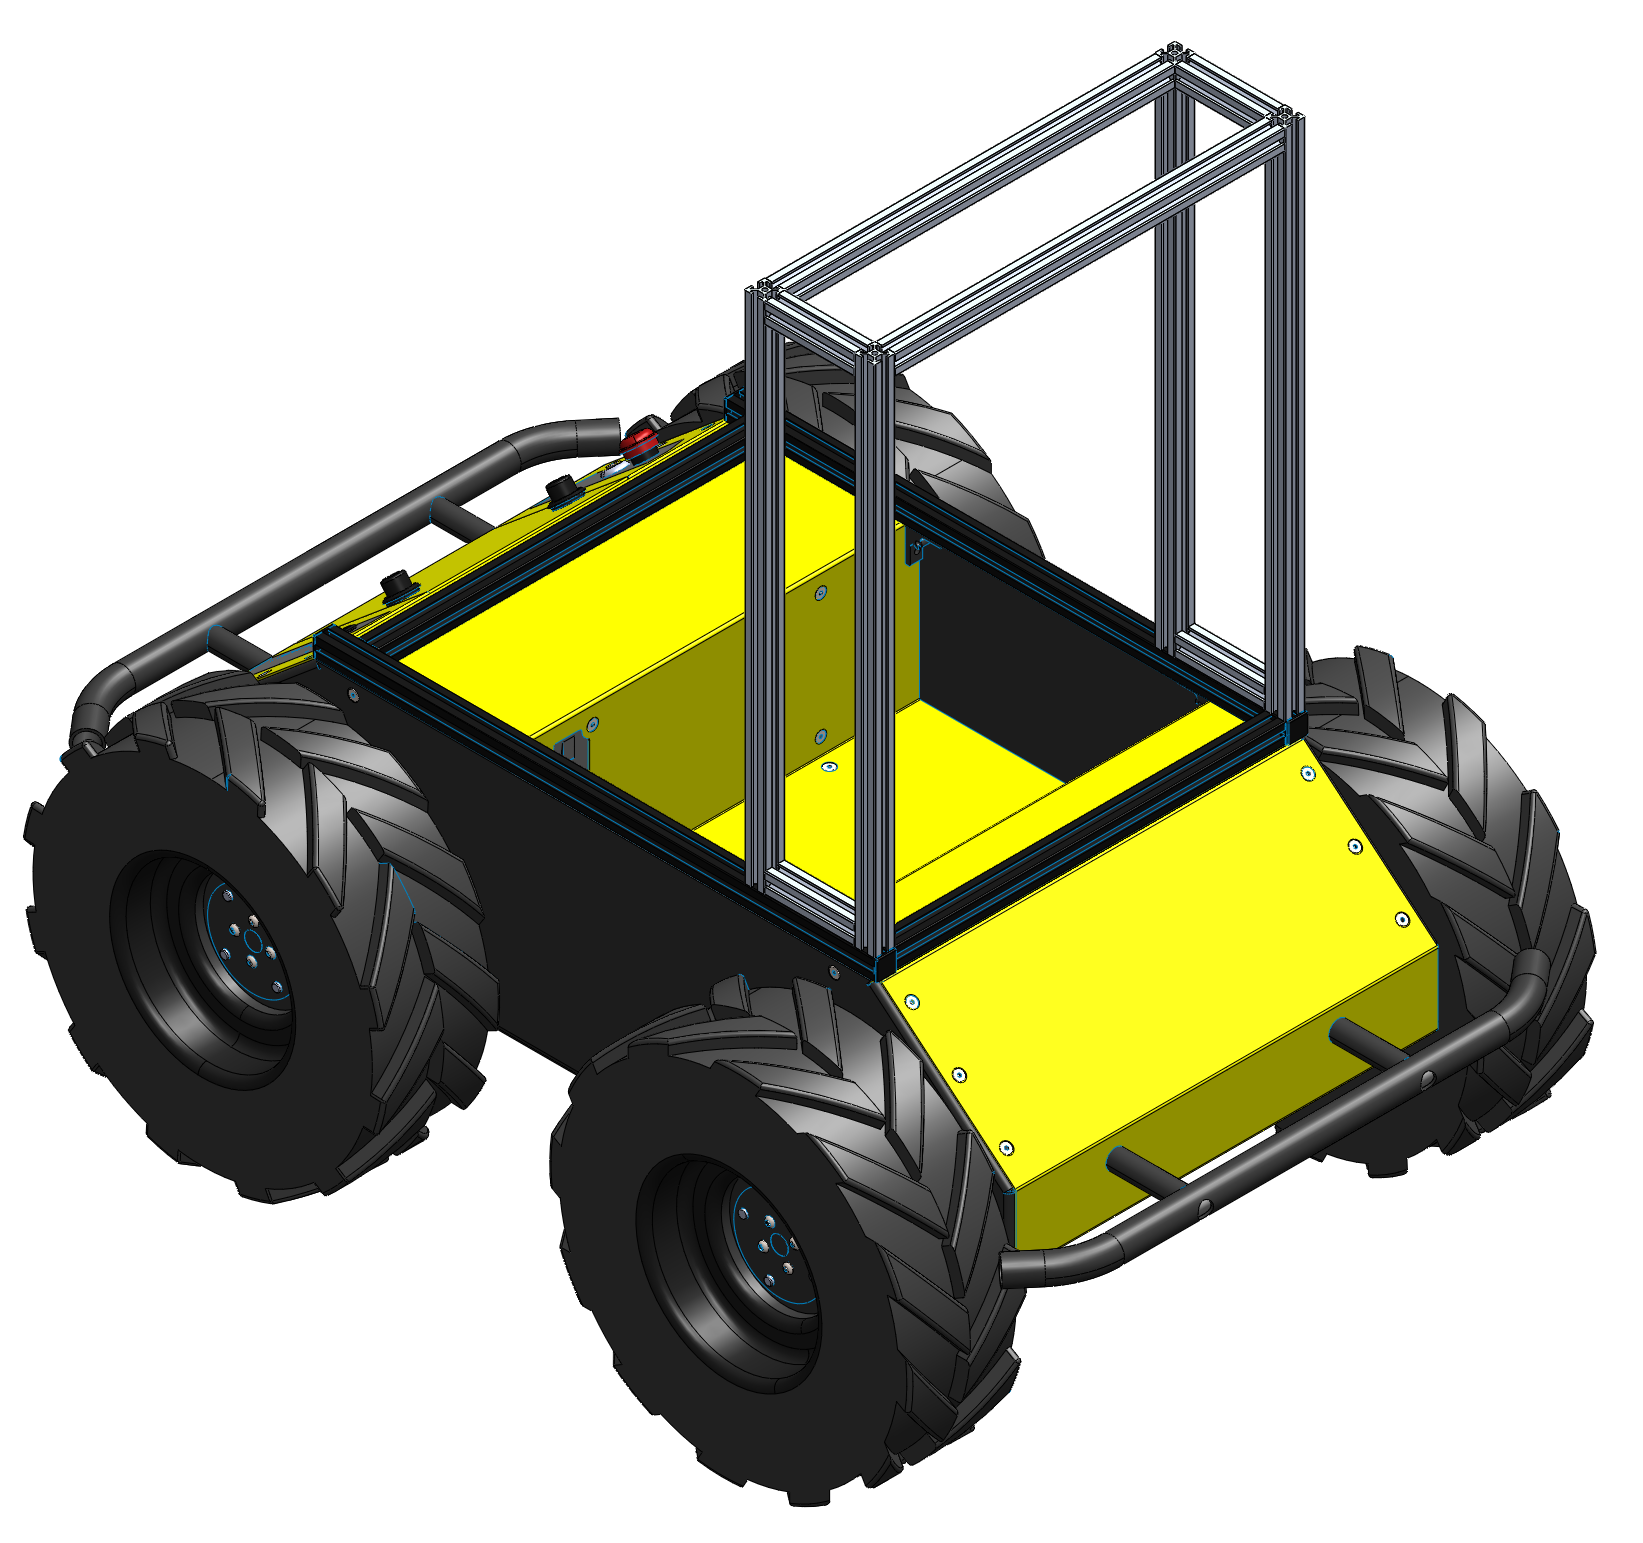
\includegraphics[width = 0.5\textwidth]{Figures/husky_with_frame.png}
  \caption{CAD model of Husky A200 with sensor frame mounted}
  \label{fig:M:H:AMF:userFrame}
\end{figure}

% \subsubsection{IMU}\label{sec:M:H:ANH:IMU}
% In order to increase the performance of the UGV odometry, an UM7 IMU from Redshift Labs, seen in figure \ref{fig:um7_imu}, has been added. This IMU is ROS2 compatible and will publish IMU data to ROS2. This data can then be used to better calculate the position of the UGV. 

% \begin{figure}[htp]
%   \centering
%   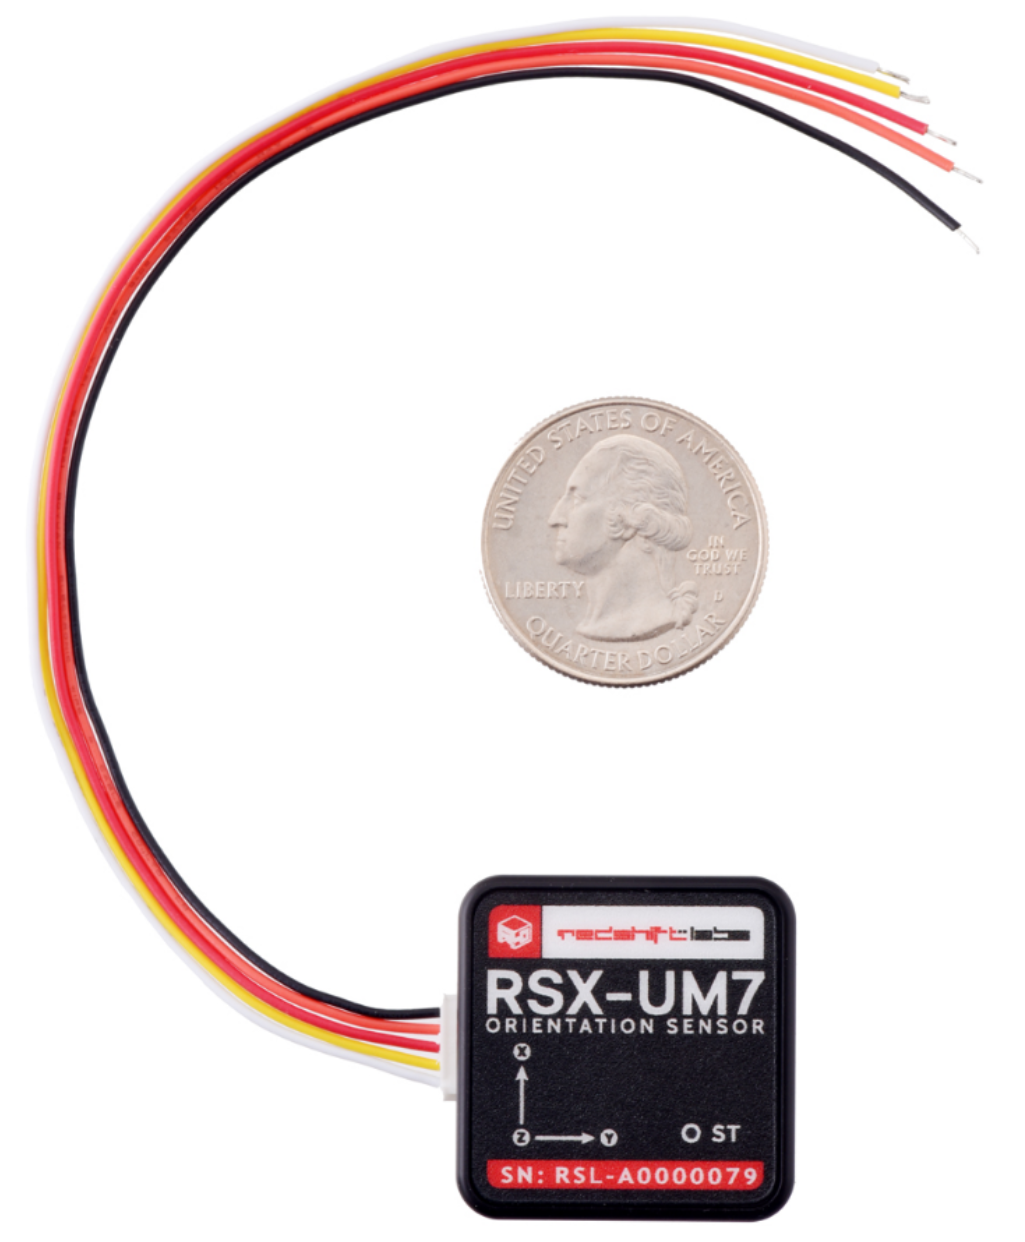
\includegraphics[width = 0.3\textwidth]{Figures/um7_imu.png}
%   \caption{Redshift Labs UM7 IMU. Image from \cite{um7_imu}.}
%   \label{fig:um7_imu}
% \end{figure}

% As illustrated in the topology in figure \ref{fig:topology}, the UM7 is connected to the UGV Xavier through USB which is used for power and communication.

% \subsection{LiDAR}\label{sec:M:H:ANH:Lidar}
% The Ouster OS1-64, is a $360\deg$ 3D LiDAR that generates a large amount of spatial information about the surrounding environment as a point cloud. In this project, that point cloud is used for localisation and to generate a 2D map of the environment. The OS1-164 LiDAR is fitted with a built in IMU sensor which for example can be used the same way, or together with, the UM7 IMU for localisation. The LiDAR can be seen mounted on a camera bracket in figure \ref{fig:lidar_mount}.

%\subsection{LiDAR and Camera Mount}\label{sec:M:H:ANH:LidarAndCameraMount}
To account for the possibility to fuse LiDAR and image data, a LiDAR and camera mount, seen in figure \ref{fig:lidar_mount}, is created. The mount is designed to have the Ouster OS1 LiDAR mounted on the top and four cameras inside. The cameras are arranged $90\deg$ away from each other with a constant radius from the center of the mount. These cameras are not further used in this thesis, the possibility to add these was added upon request, to allow for LiDAR-Camera fusion.

%\subsection{Pick and Place Hardware}\label{sec:M:H:PickandPlaceHardware}

%\subsubsection{Manipulator}\label{sec:M:H:P&PH:Manipulator}

%\subsubsection{Manipulator Mounted Camera}\label{sec:M:H:P&PH:ManipulatorMountedCamera}
The Intel Realsense D435i camera is mounted on the manipulator by a bracket designed in CAD software. The bracket is adapted from \cite{d435_sleeve}, with modifications to be able to mount it on the gripper of the V300 manipulator. The bracket can be seen in figure \ref{fig:realsense_assembly}.

\begin{figure}[htp]
  \centering
  \begin{minipage}[b]{0.49\textwidth}
    \centering
    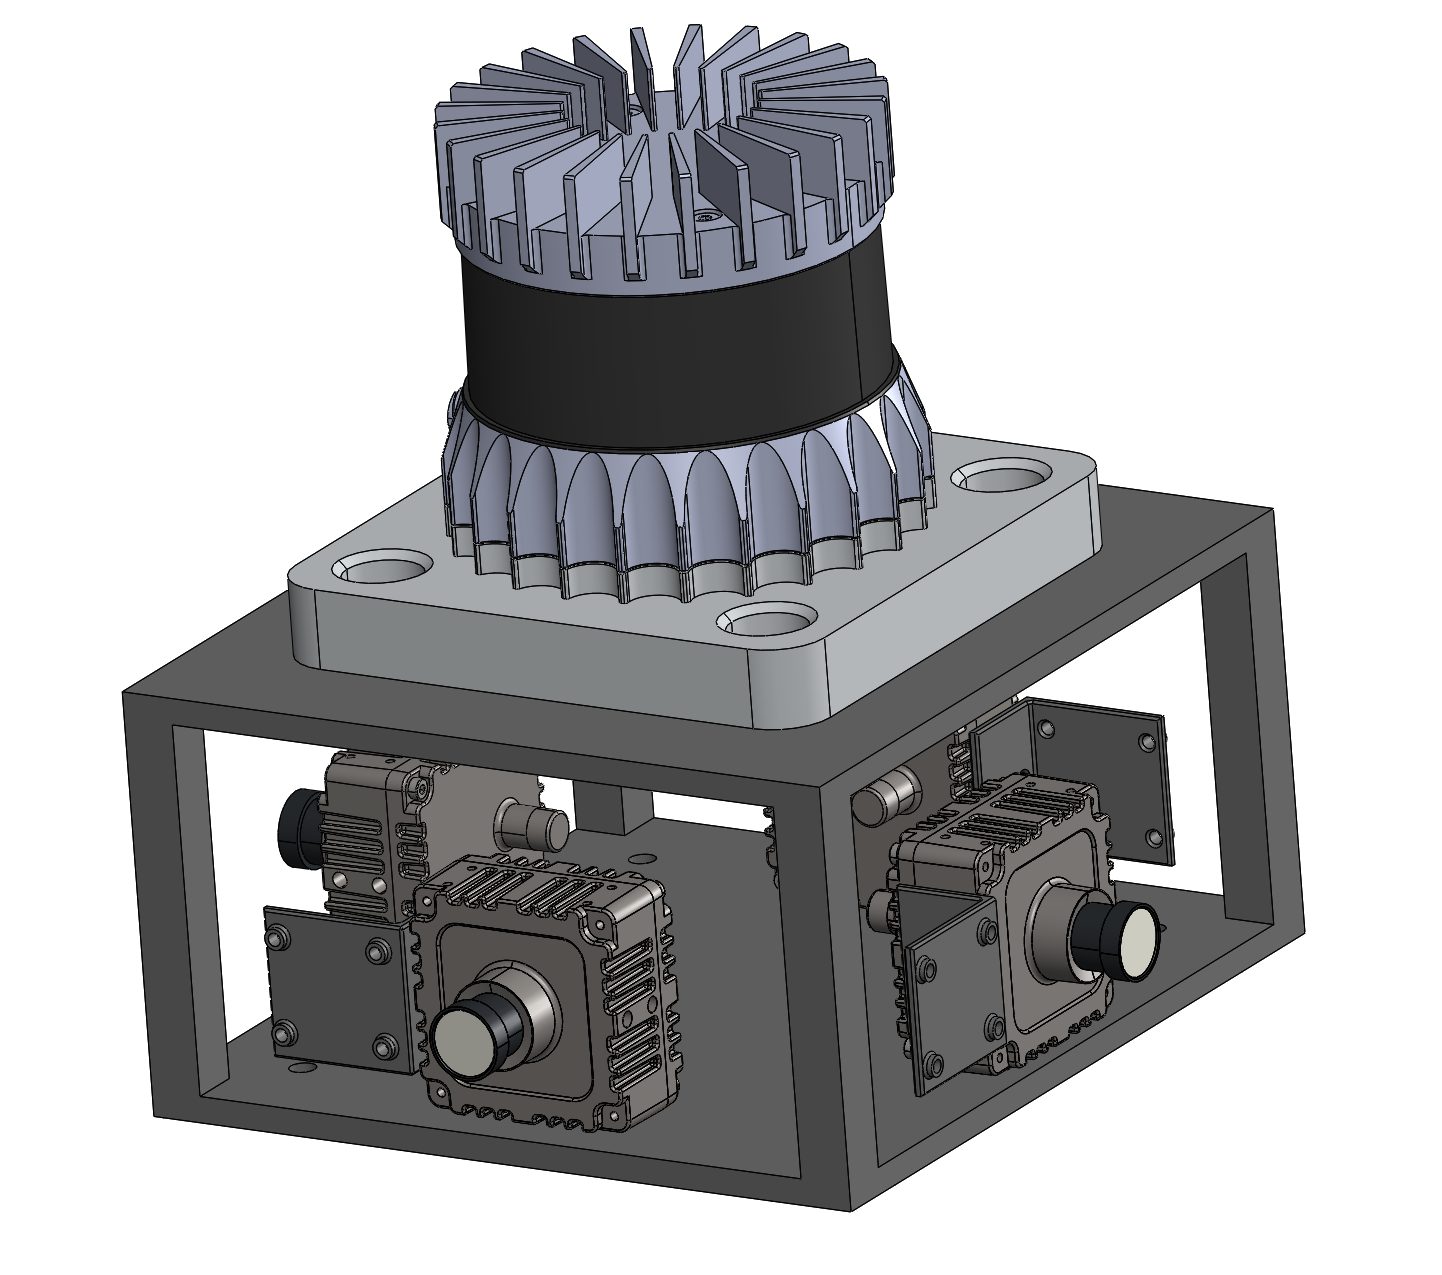
\includegraphics[width = 0.8\textwidth]{Figures/lidar_mount.png}
    \caption{Cad model of LiDAR mount with cameras. The Ouster OS1-64 is mounted on top.}
     \label{fig:lidar_mount}
  \end{minipage}
  \hfill
  \begin{minipage}[b]{0.49\textwidth}
    \centering
    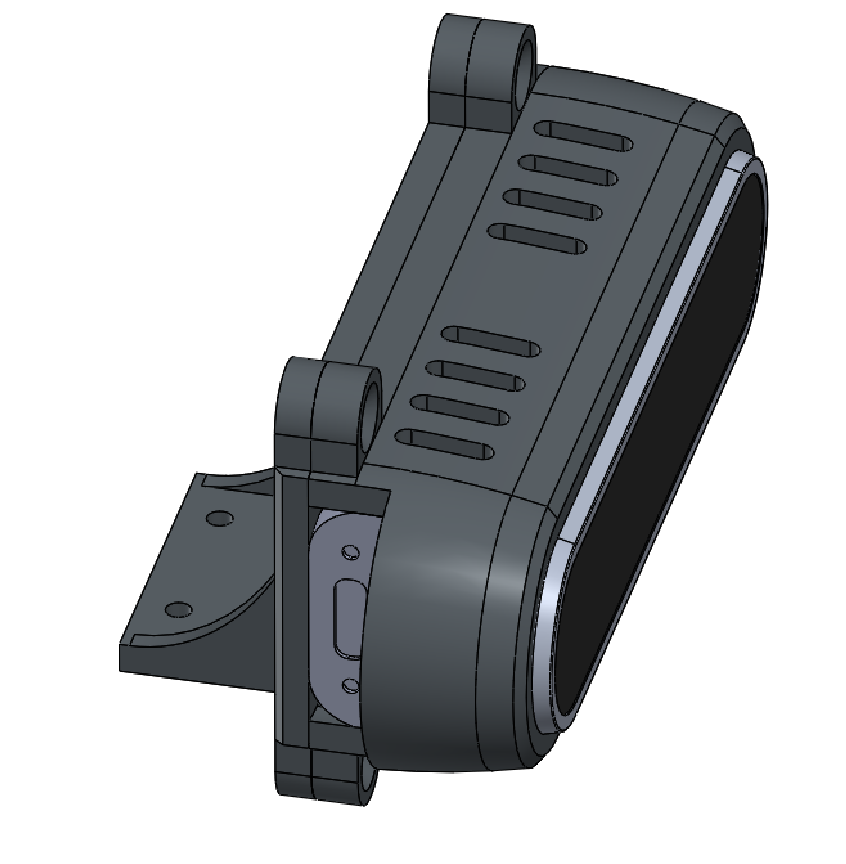
\includegraphics[width = 0.8\textwidth]{Figures/realsense_assembly.pdf}
    \caption{Realsense D435i bracket assembly with camera. The bracket is adapted from \cite{d435_sleeve} to be able to mount on the VX300 robotic arm.}
    \label{fig:realsense_assembly}
  \end{minipage}
\end{figure}

% \begin{figure}[htp]
%   \centering
%   \begin{minipage}[b]{0.49\textwidth}
%     \centering
%     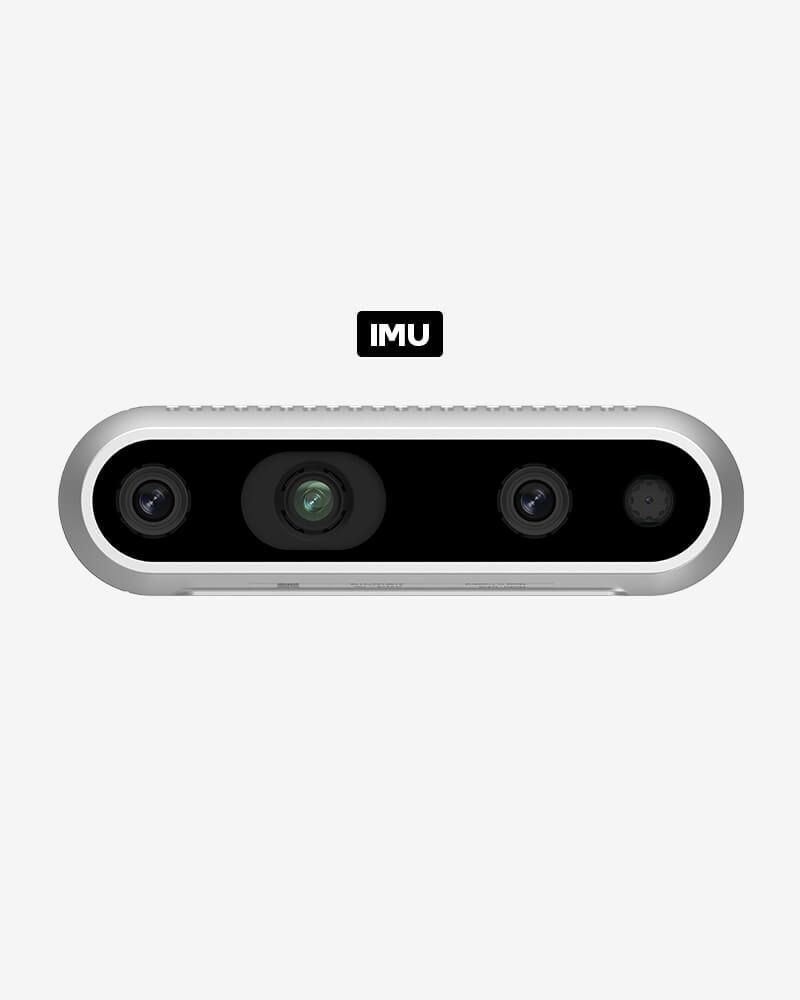
\includegraphics[width = 0.8\textwidth]{Figures/D435i.jpg}
%     \caption{Intel Realsense D435i Depth Camera. Image from: \cite{realsense_d435i}.}
%     \label{fig:d435i}
%   \end{minipage}
%   \hfill
%   \begin{minipage}[b]{0.49\textwidth}
%    \centering
%     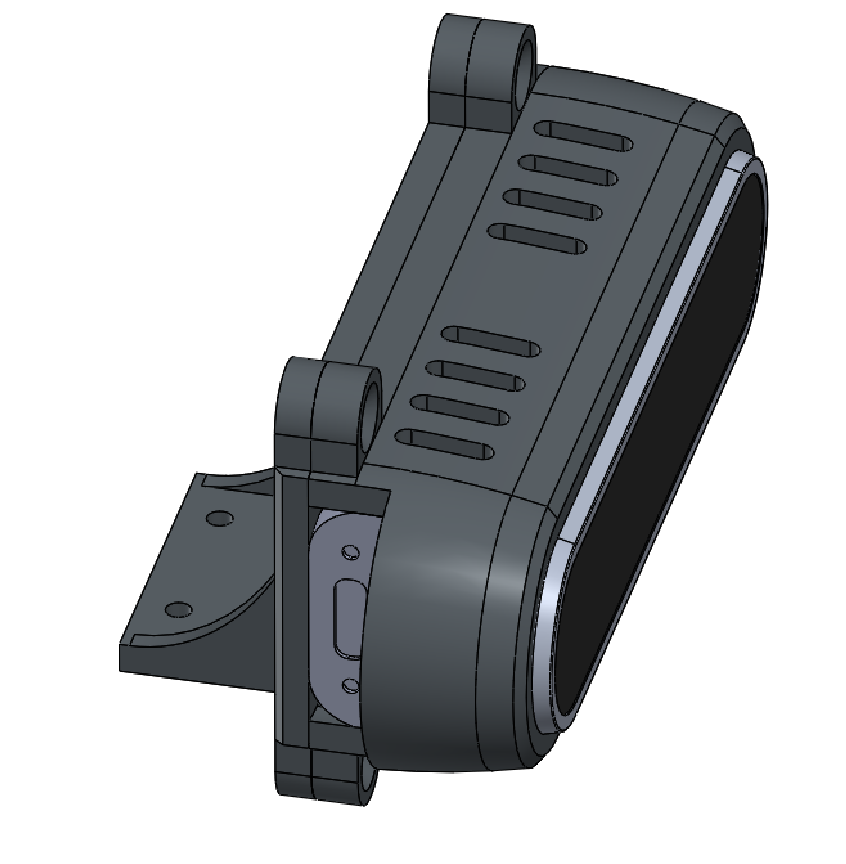
\includegraphics[width = 0.8\textwidth]{Figures/realsense_assembly.pdf}
%     \caption{Realsense D435i bracket assembly with camera. The bracket is adapted from \cite{d435_sleeve} to be able to mount on the VX300 robotic arm.}
%     \label{fig:realsense_assembly}
%   \end{minipage}
% \end{figure}

\subsection{Complete Hardware Configuration}
The complete hardware configuration is presented as a CAD model in figure \ref{fig:M:H:CHS:CadHuskyComplete}. The figure illustrates how the accessory mounting frame along with the camera mount is added to the front of the UGV. The manipulator can be seen mounted on the aluminium profiles at the rear right side of the UGV. Offsetting the base of the manipulator from the center of the UGV, gives a longer reach outside of the UGV's footprint. The actual experimental setup is presented in figure \ref{fig:M:H:CHS:PhysHuskyComplete}. The WiFi router described in the beginning of section \ref{sec:M:Hardware}, can be seen mounted at the front of the accessory mounting frame in figure \ref{fig:M:H:CHS:PhysHuskyComplete}. This is in accordance with the general arrangement drawing.

\begin{figure}[htp]
  \centering
  \begin{minipage}[b]{0.49\textwidth}
    \centering
    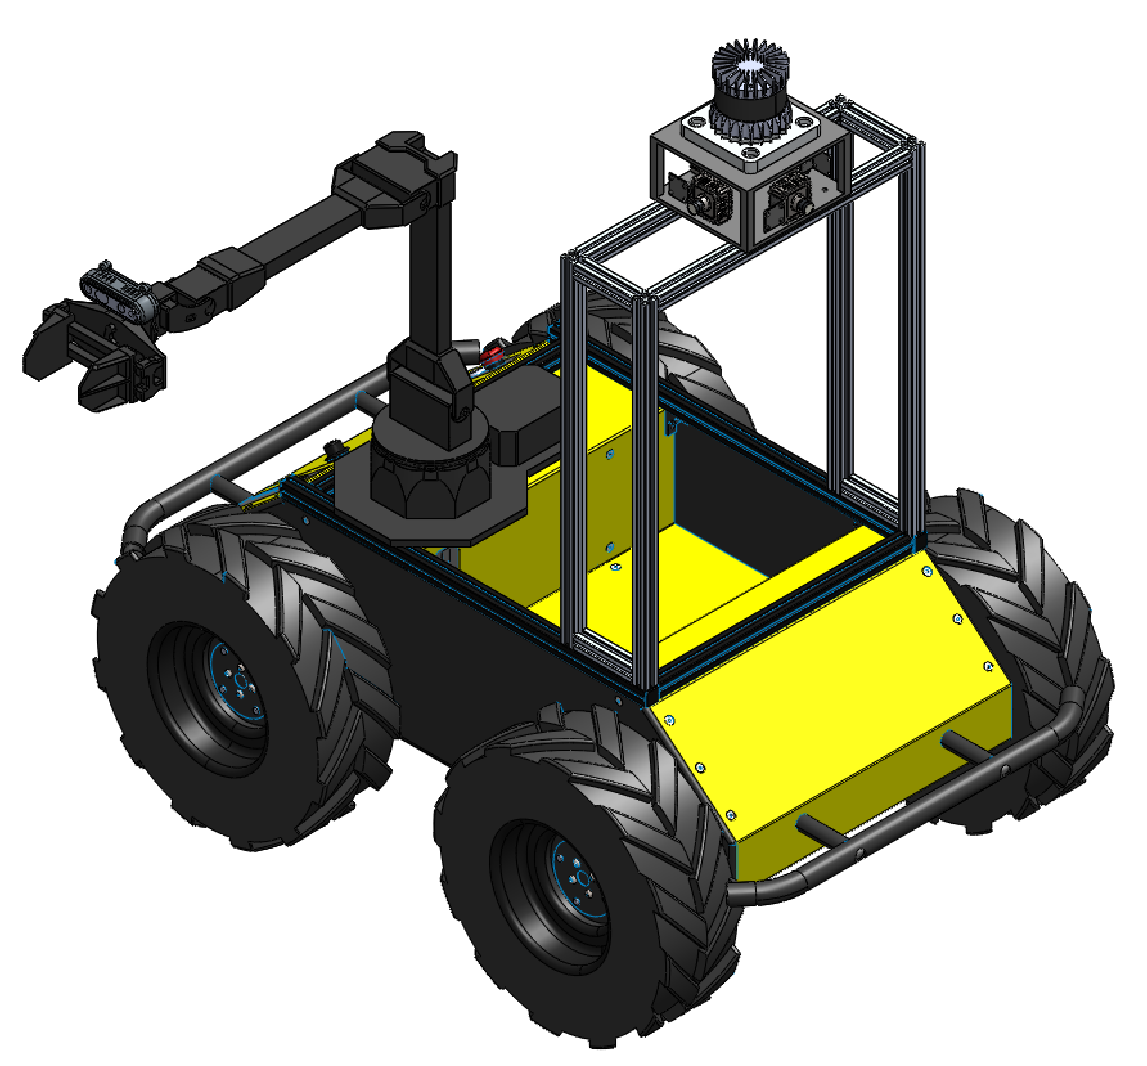
\includegraphics[width = 0.8\textwidth]{Figures/husky_completed.pdf}
    \caption{3D CAD model of the complete robotic system. The accessory mounting frame with the LiDAR mount and the LiDAR is modelled on top of the Husky A200 UGV platform. The VX300 manipulator with it's RealSense D435i camera is mounted at the rear right corner of the UGV platform.}
    \label{fig:M:H:CHS:CadHuskyComplete}
  \end{minipage}
  \hfill
  \begin{minipage}[b]{0.49\textwidth}
    \centering
    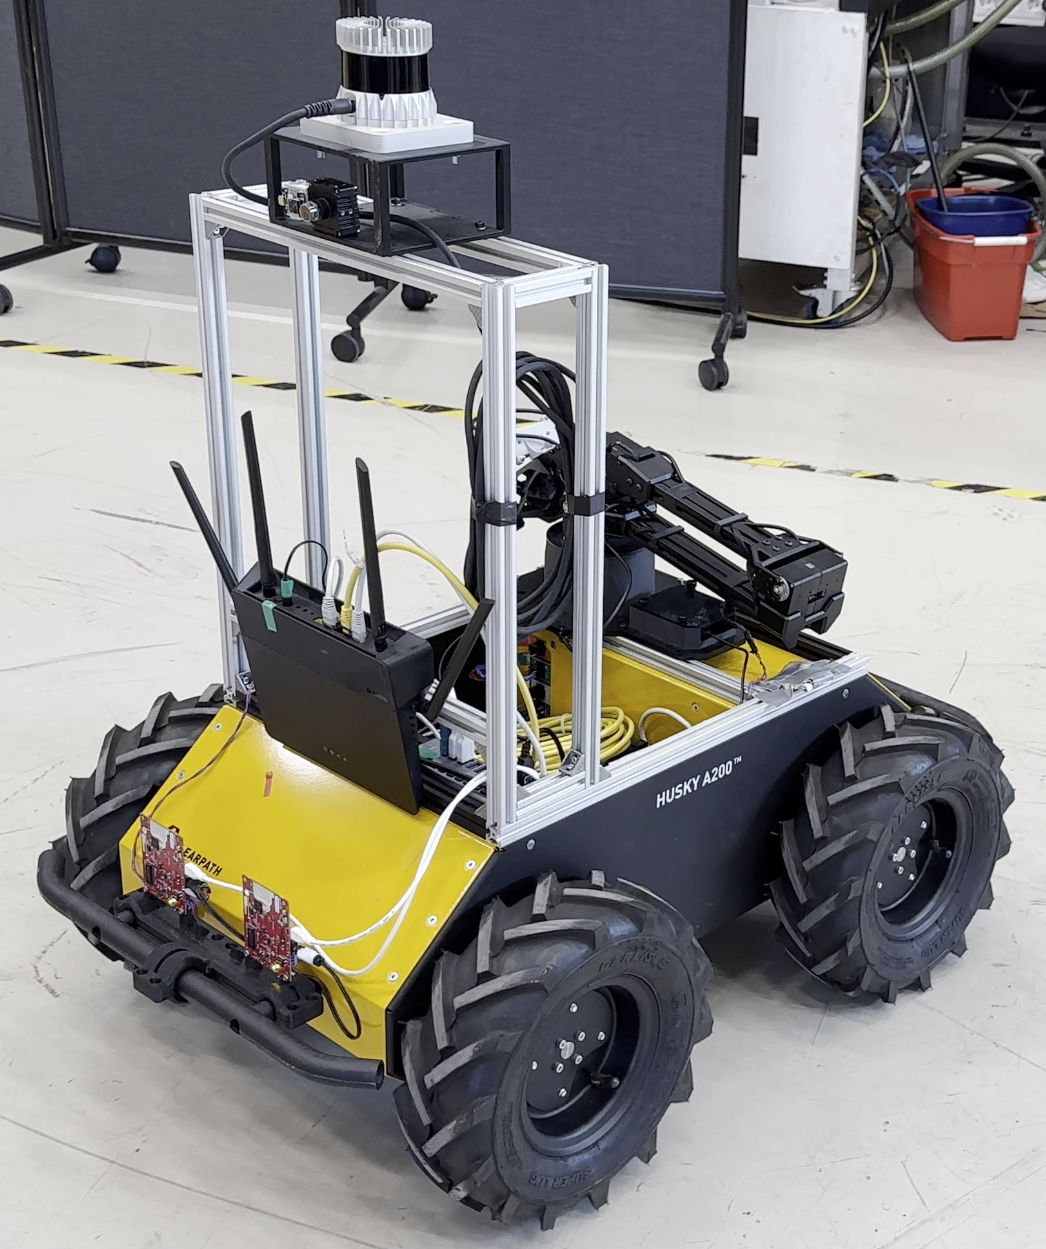
\includegraphics[width = 0.8\textwidth]{Figures/figHuskyComplete.png}
    \caption{Complete experimental robotic system. The accessory mounting frame can be seen mounted on the Husky A200 UGV with the LiDAR mount including the OS1 LiDAR on top. Additionally, it can be seen that the VX300 manipulator is mounted in the rear right corner of the UGV.}
    \label{fig:M:H:CHS:PhysHuskyComplete}
  \end{minipage}
\end{figure}

A closer look at the experimental manipulator setup with it's mounted Realsense D435i camera is presented in figure \ref{fig:M:H:M:M:MMC:Vx300Complete}.

\begin{figure}[H]
  \centering
  \begin{minipage}[b]{0.49\textwidth}
        \centering
        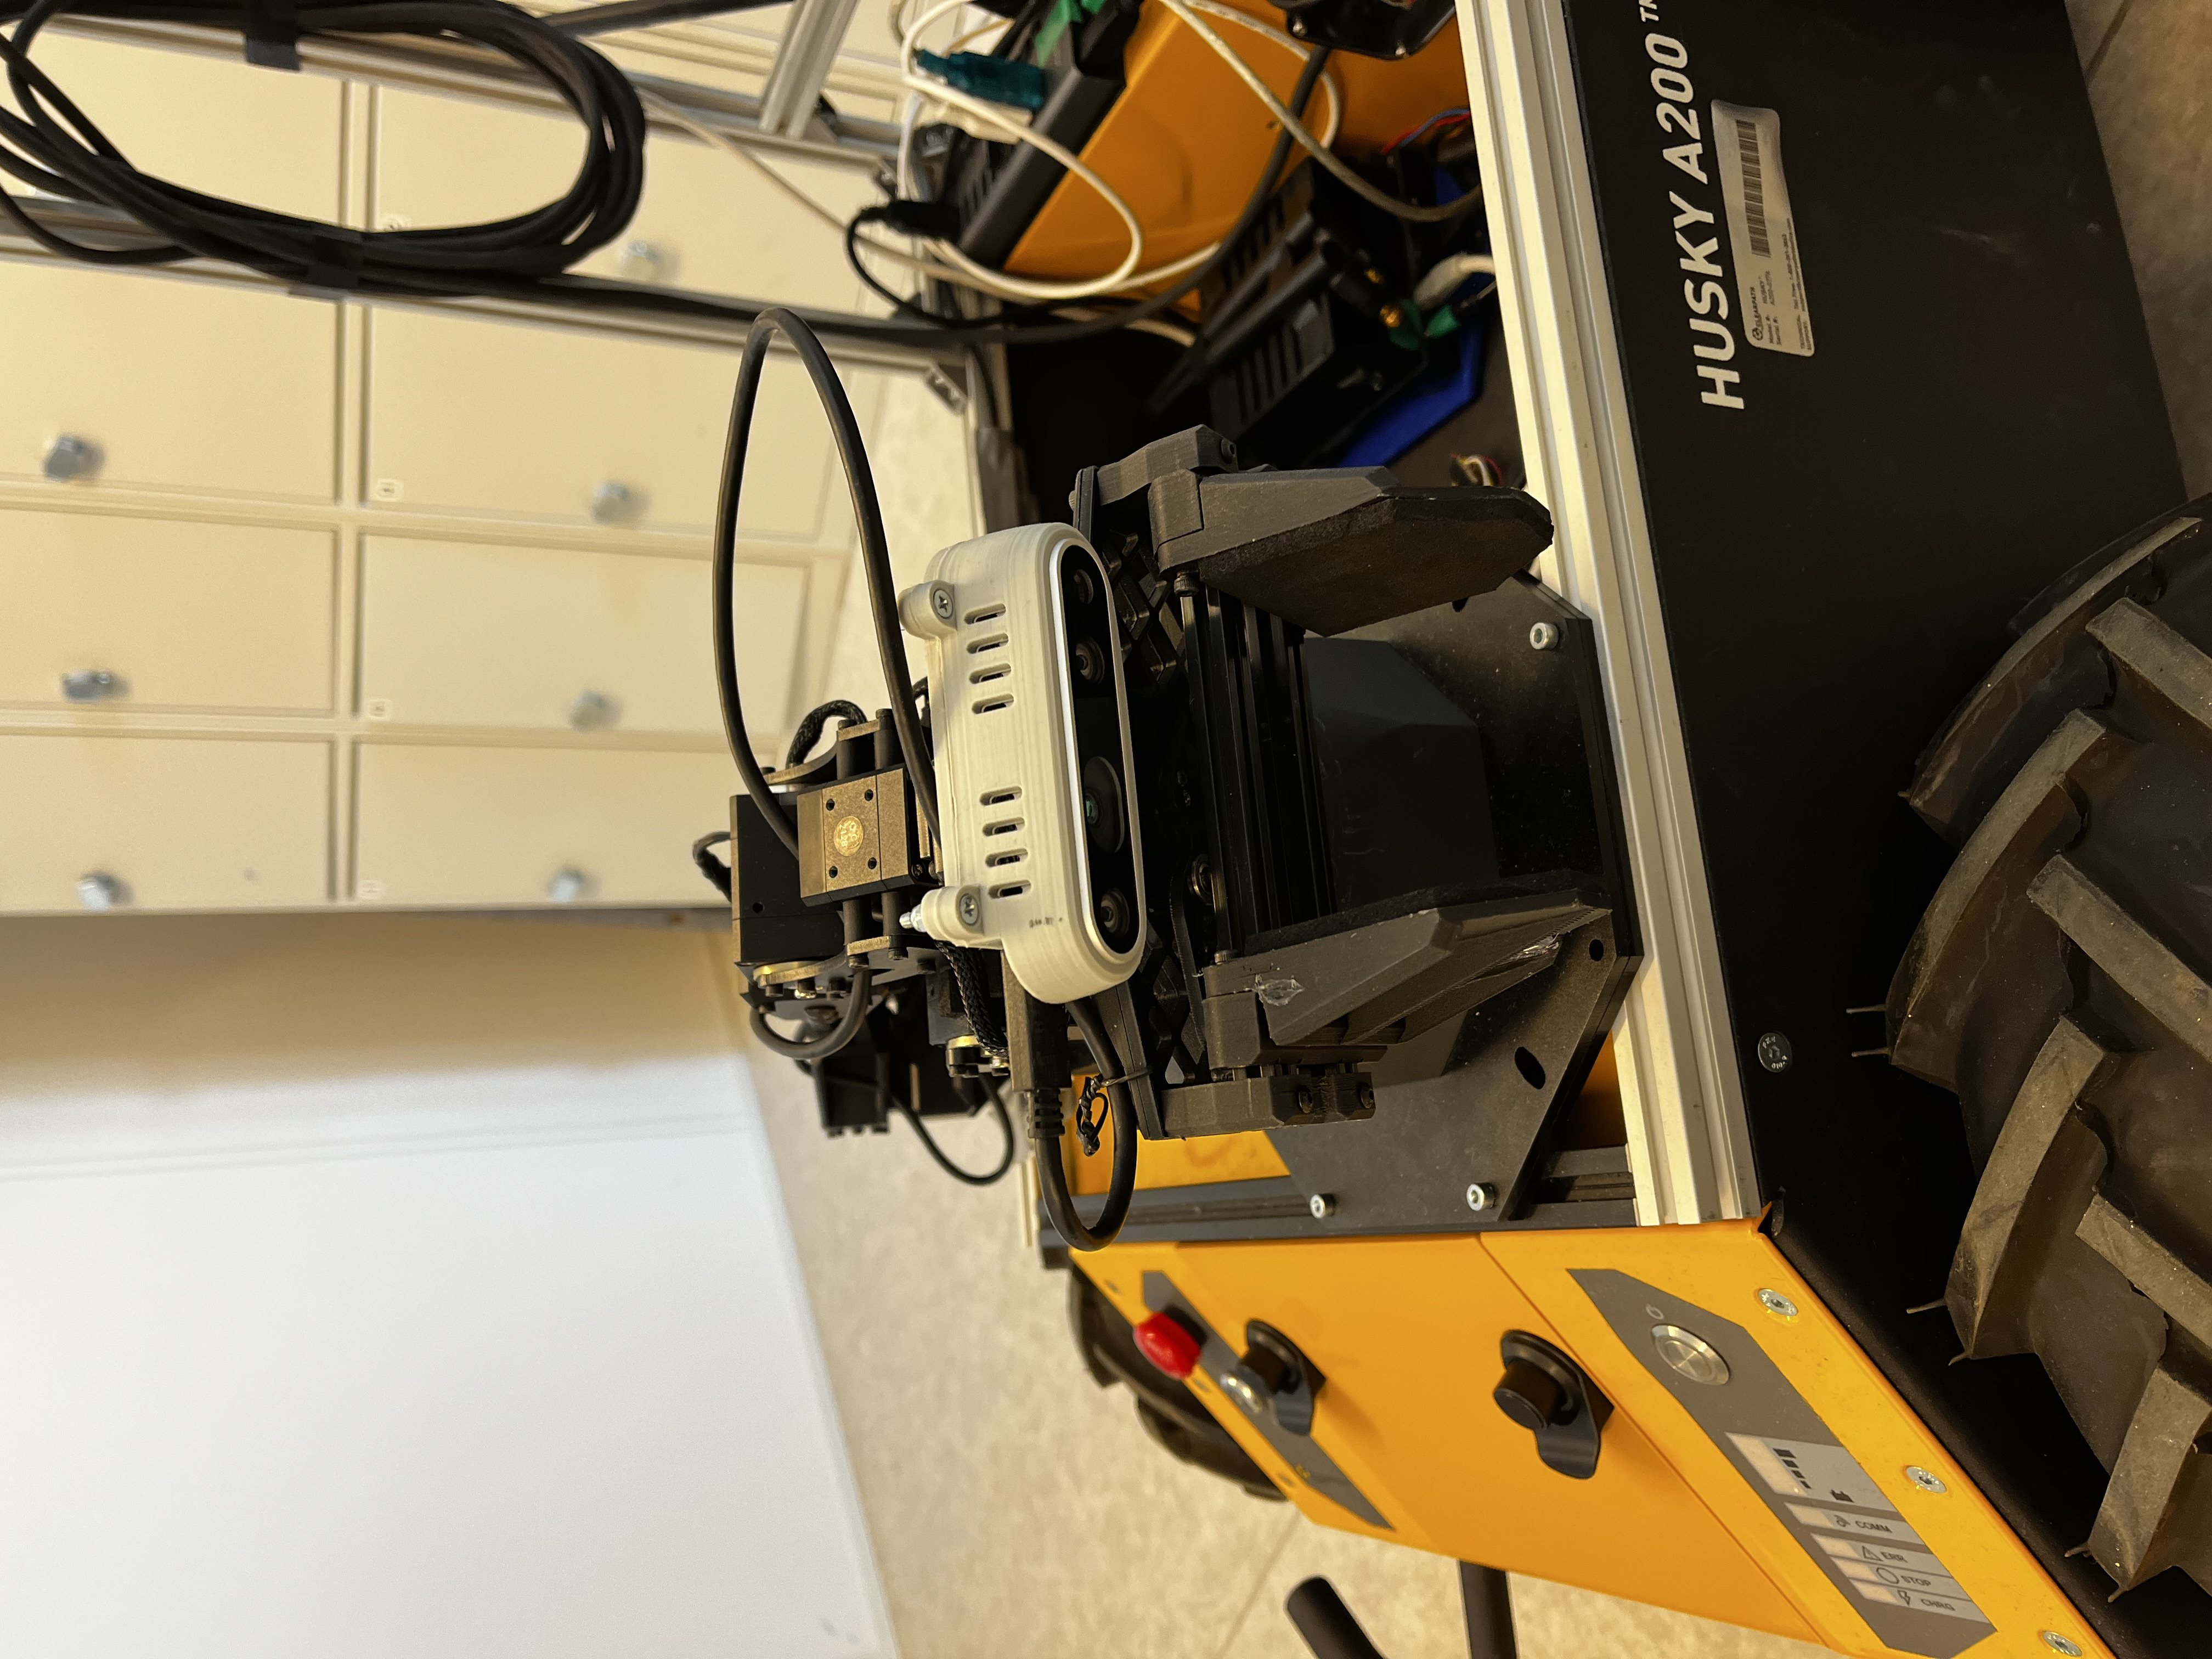
\includegraphics[angle=-90,width = 0.8\textwidth]{Figures/figVX300PhysComplete1.jpg}
  \end{minipage}
  \hfill
  \begin{minipage}[b]{0.49\textwidth}
    \centering
    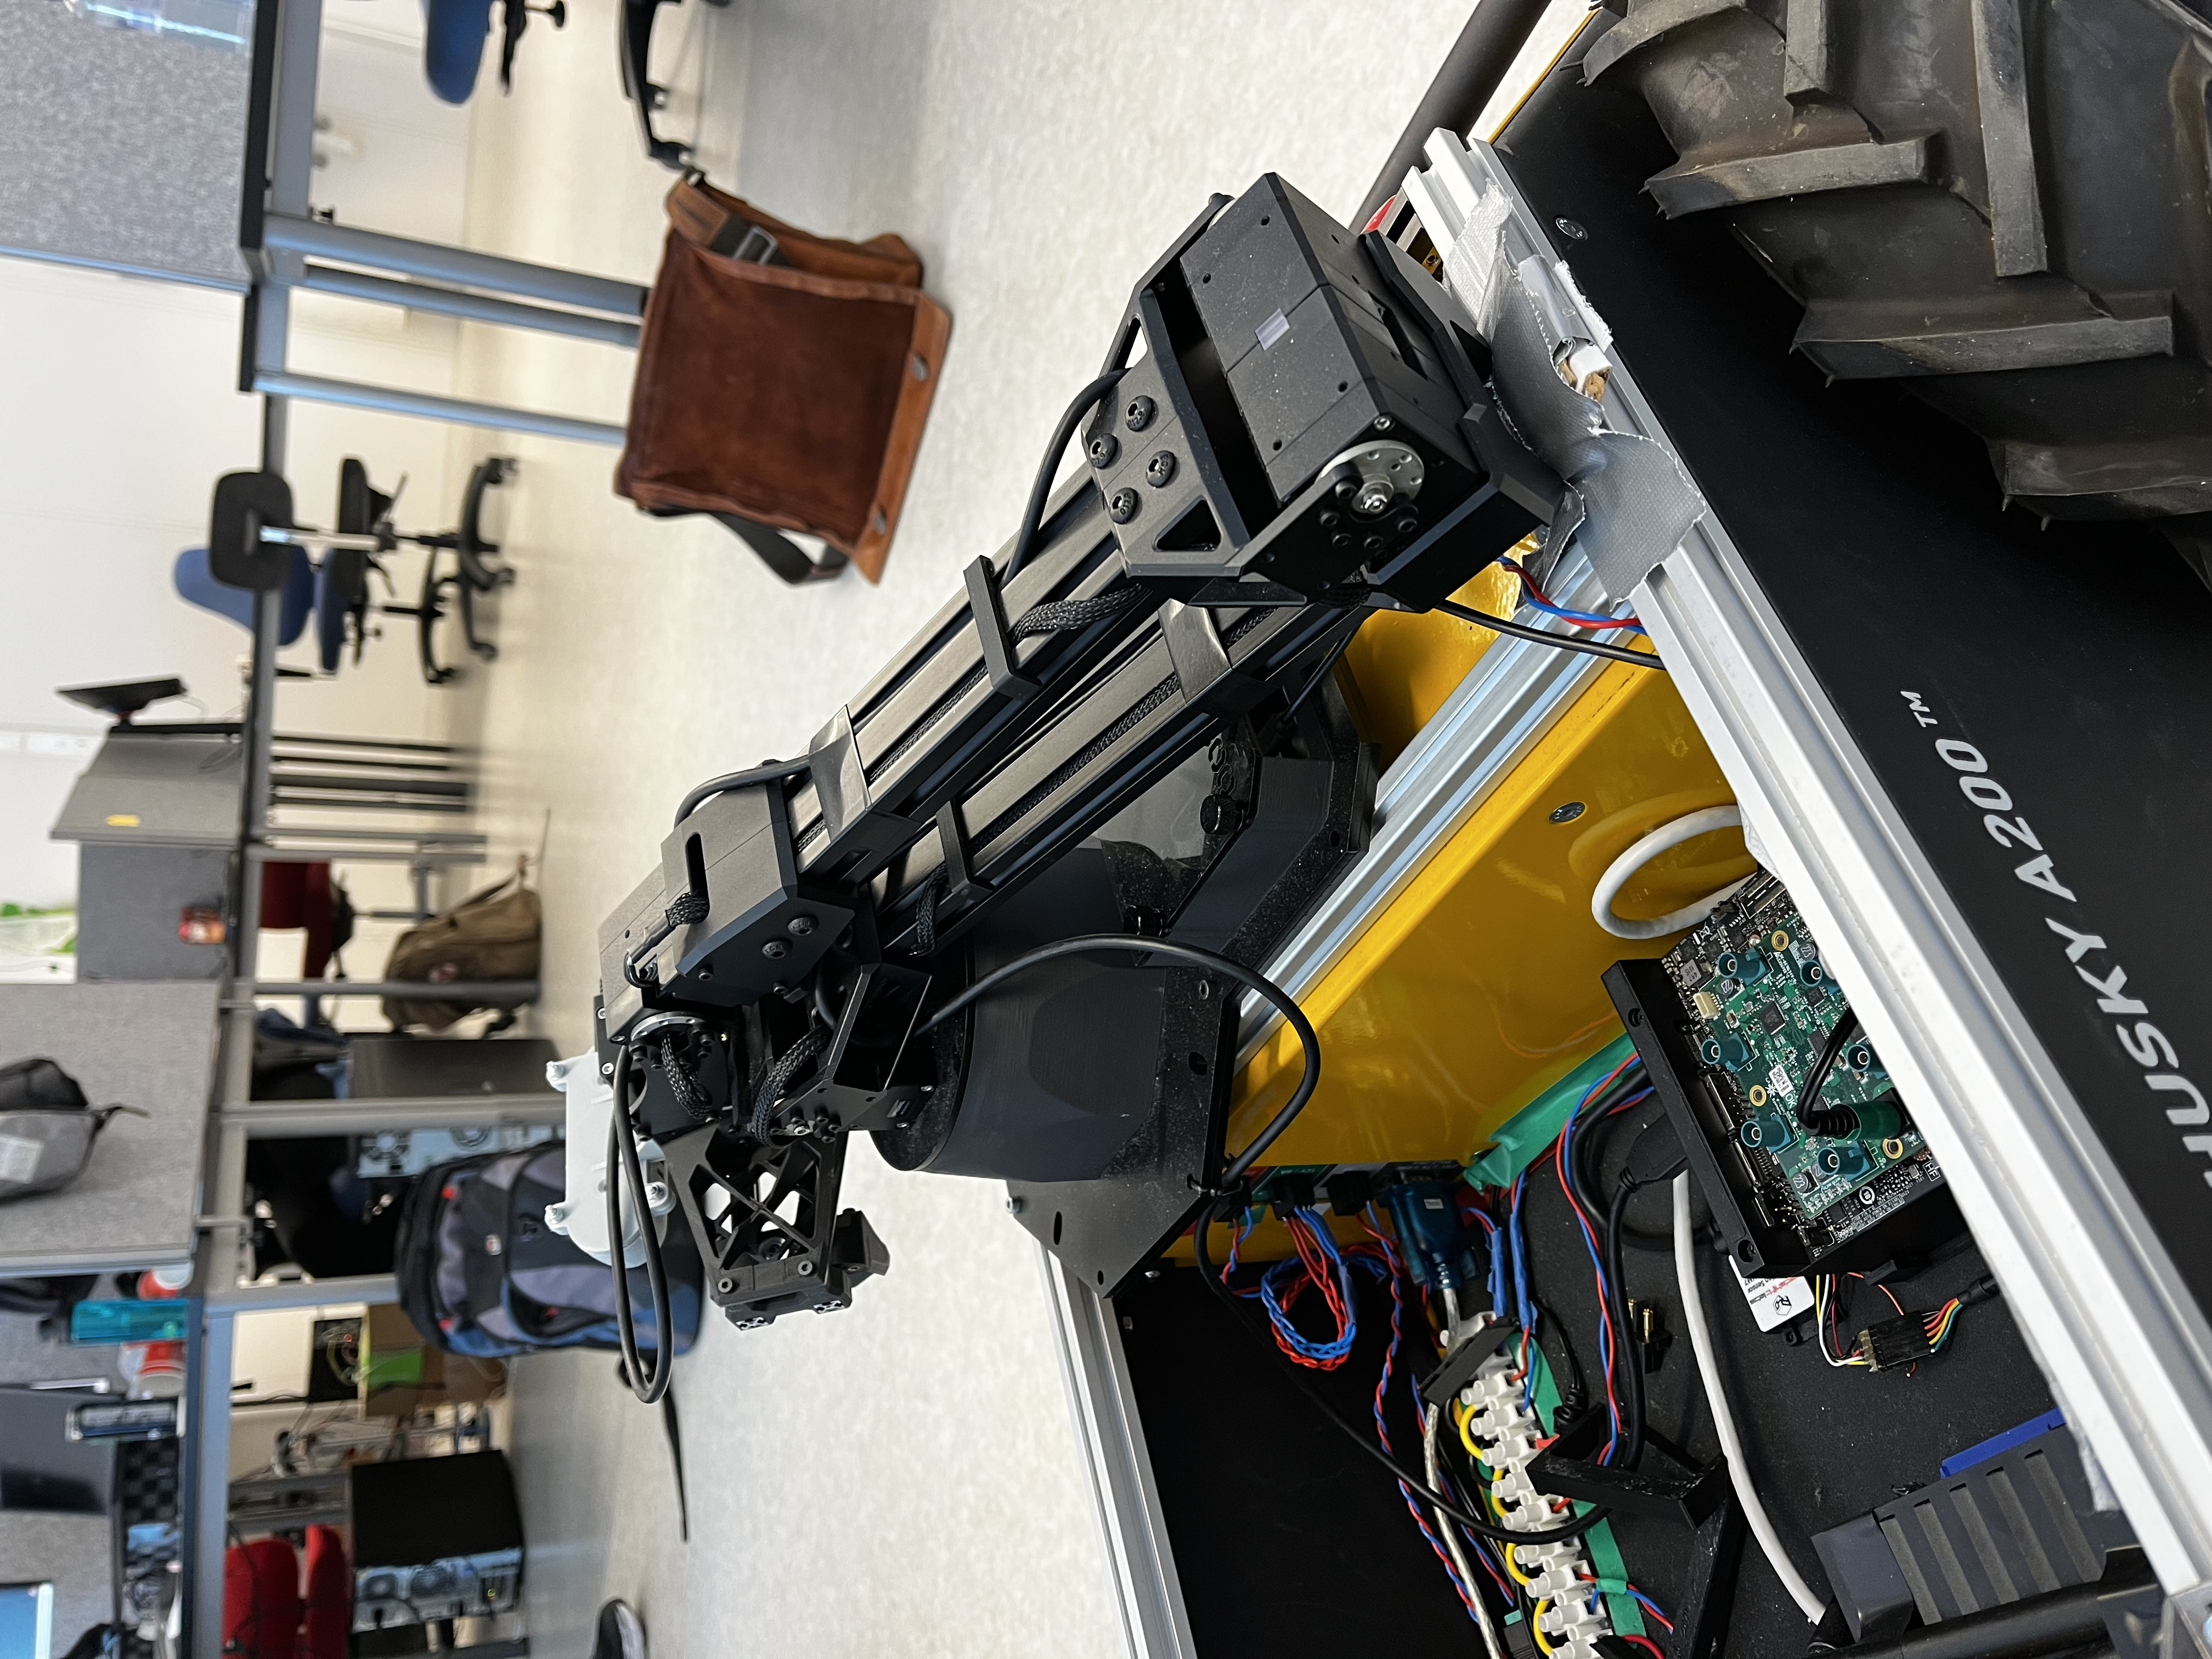
\includegraphics[angle=-90,width = 0.8\textwidth]{Figures/figVX300PhysComplete5.jpg}
  \end{minipage}
  \caption{Interbotix VX300 manipulator mounted on the Husky A200 UGV along with the manipulator mounted Realsense D435i camera. The Manipulator, although powered off in the image, receives it's power through the UGV's 12V power supply and controlled via an on-board Nvidia Jetson AGX Xavier Computer.}
  \label{fig:M:H:M:M:MMC:Vx300Complete}
\end{figure}


% \section{Mobile Robot Configuration}
% For the different components of the robotic system to act together, some software configuration has to be done. This section describes different  parts of the software setup to achieve an autonomously navigating robotic platform. As mentioned in \textbf{HERE, I HAVE TO MENTION A SECTION} ROS2 is used for software implementation. All ROS2 packages described in this section is either available as open source packages, or developed during the course of this project.


\section{Autonomous Navigation} \label{sec:M:AutonomousNavigation}
An overview of the autonomous navigation system is illustrated at a high level in figure \ref{fig:M:AN:ANMethod}. This figure shows the relation between the different subsystems that make up this navigation system and what kind of information that are transmitted between them. The figure is divided into four parts in correspondence to the description in section \ref{sec:T:AutonomousNavigation}. These four parts are Motion Control, Perception, Localisation and Mapping and Navigation. 

\begin{figure}[htp]
  \centering
  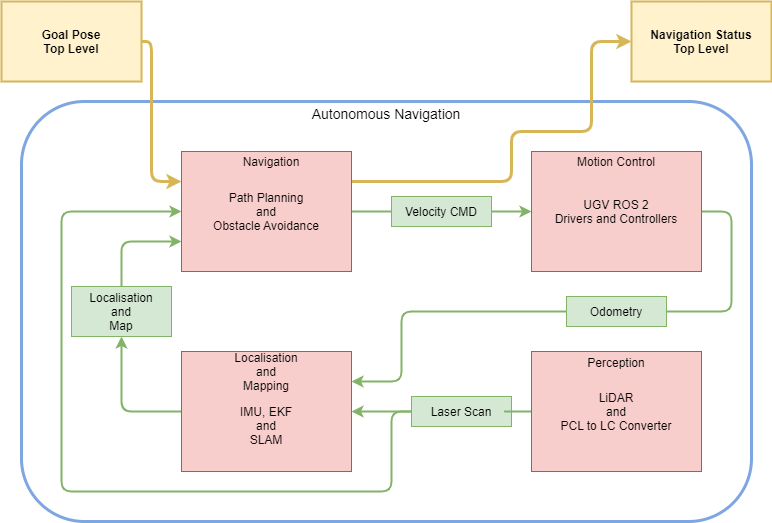
\includegraphics[width = 0.98\textwidth]{Figures/figANMethod.drawio.png}
  \caption{Overview of autonomous navigation system. Motion Control provides odometry information, which is fused with IMU data in an EKF. The resulting filtered odometry is fed to SLAM along with Laser Scan from a LiDAR. SLAM then provides mapping and localisation for the navigation system. Path planning and collision avoidance is preformed in the navigation system which sends command velocities to the motion control system based on info.}
  \label{fig:M:AN:ANMethod}
\end{figure}
% Aj fig not redable. increas the fontzize and make blocks compact. need to discuss this to understand and how it can be explained better

Motion Control regards the controllers that takes care of the movement of the UGV\textbf{SAy WHAT MC IN METHOD REGARDS}. As seen in figure \ref{fig:M:AN:ANMethod}, motion control takes in velocity commands. It then acts upon these and calculates odometry based on it's resulting movement.

The perception system in this project, consists of the Ouster OS1-64 LiDAR and a PointCloud to LaserScan converter. The point cloud from the OS1 LiDAR is passed to this converter, which converts the relevant information into a 2 dimensional laser scan.

The odometry coming from motion control passes into the EKF, which is a part of the Localisation and Mapping subsystem. As seen in figure \ref{fig:M:AN:ANMethod}, EKF also takes in IMU data from both the UM7 IMU and the Ouster OS1 LiDAR. It then fuses all this information in order to optimise the odometry estimate of the robot. This "filtered odometry" is then passed into the SLAM algorithm along with laser scan from the perception system. The SLAM algorithm uses this information to construct a 2D map of the environment and estimate the robots position in the map. 

Finally, the navigation subsystem use the information from SLAM and Perception to preform path planning and obstacle avoidance. The navigation subsystem is also the one that interacts with the top level system by taking pose goals as commands and providing feedback when the goal has been reached.

\subsection{Motion Control}\label{sec:M:AN:MotionControl}
As described in section \ref{sec:M:AutonomousNavigation}, motion control regards the controller of the UGV. Specifically, this is the part of the system that sets up the Husky A200 UGV towards ROS 2 so that it is able to take velocity commands through the ROS 2 network. This is done through the official ROS 2 Foxy packages provided by Clearpath \cite{husky_repo}.

% Though, Clearpath husky provides Debian ROS2 packages for ROS2 Foxy, and these are therefore used. The story is different for ROS2 Galactic which has reached its EOL and is no longer maintained. Nevertheless, the official Husky ROS2 repository\cite{husky_repo} still contains a branch for ROS2 Galactic even though it won't build. This branch is forked and modified in order to build as well as modified to take in some arguments to the launch file. The forked repository is public and available at \cite{uia_husky_repo}. 
%aj explain this - husky: foxy, SLAM: galactic, NAV2: Galactic.
%Manpulator: galactic, realsense: galactic, Apriltag: galactic
%Only Mobile robot stuff is foxy. aka, Husky, Ouster Lidar, IMU, pointcloud to laserscan
% to run two different ROS2 version modification was made and give link to your git.

It is essential for the robotic system to know the pose of the Ouster LiDAR and the UM7 IMU relative to the UGV in order to have usable sensor information. This is done through Unified Robot Description Format (URDF), which is an XML specification used to model multibody systems. At a minimum, the geometric relation between different bodies is described in URDF files. However, these may also contain inertial properties, visual properties and collision boxes. In the case of this project, the auxiliary components related to autonomous navigation is added to a URDF-file and passed upon launch of the UGV. This gives a more accurate visual representation of the robot when it is viewed in ROS 2's visual presentation software Rviz2 or ROS 2's simulation software Gazebo. Figure \ref{fig:M:AN:MC:digitalTwin} illustrates how the resulting digital twin of the mobile robot appears in Rviz2.

\begin{figure}[htp]
  \centering
  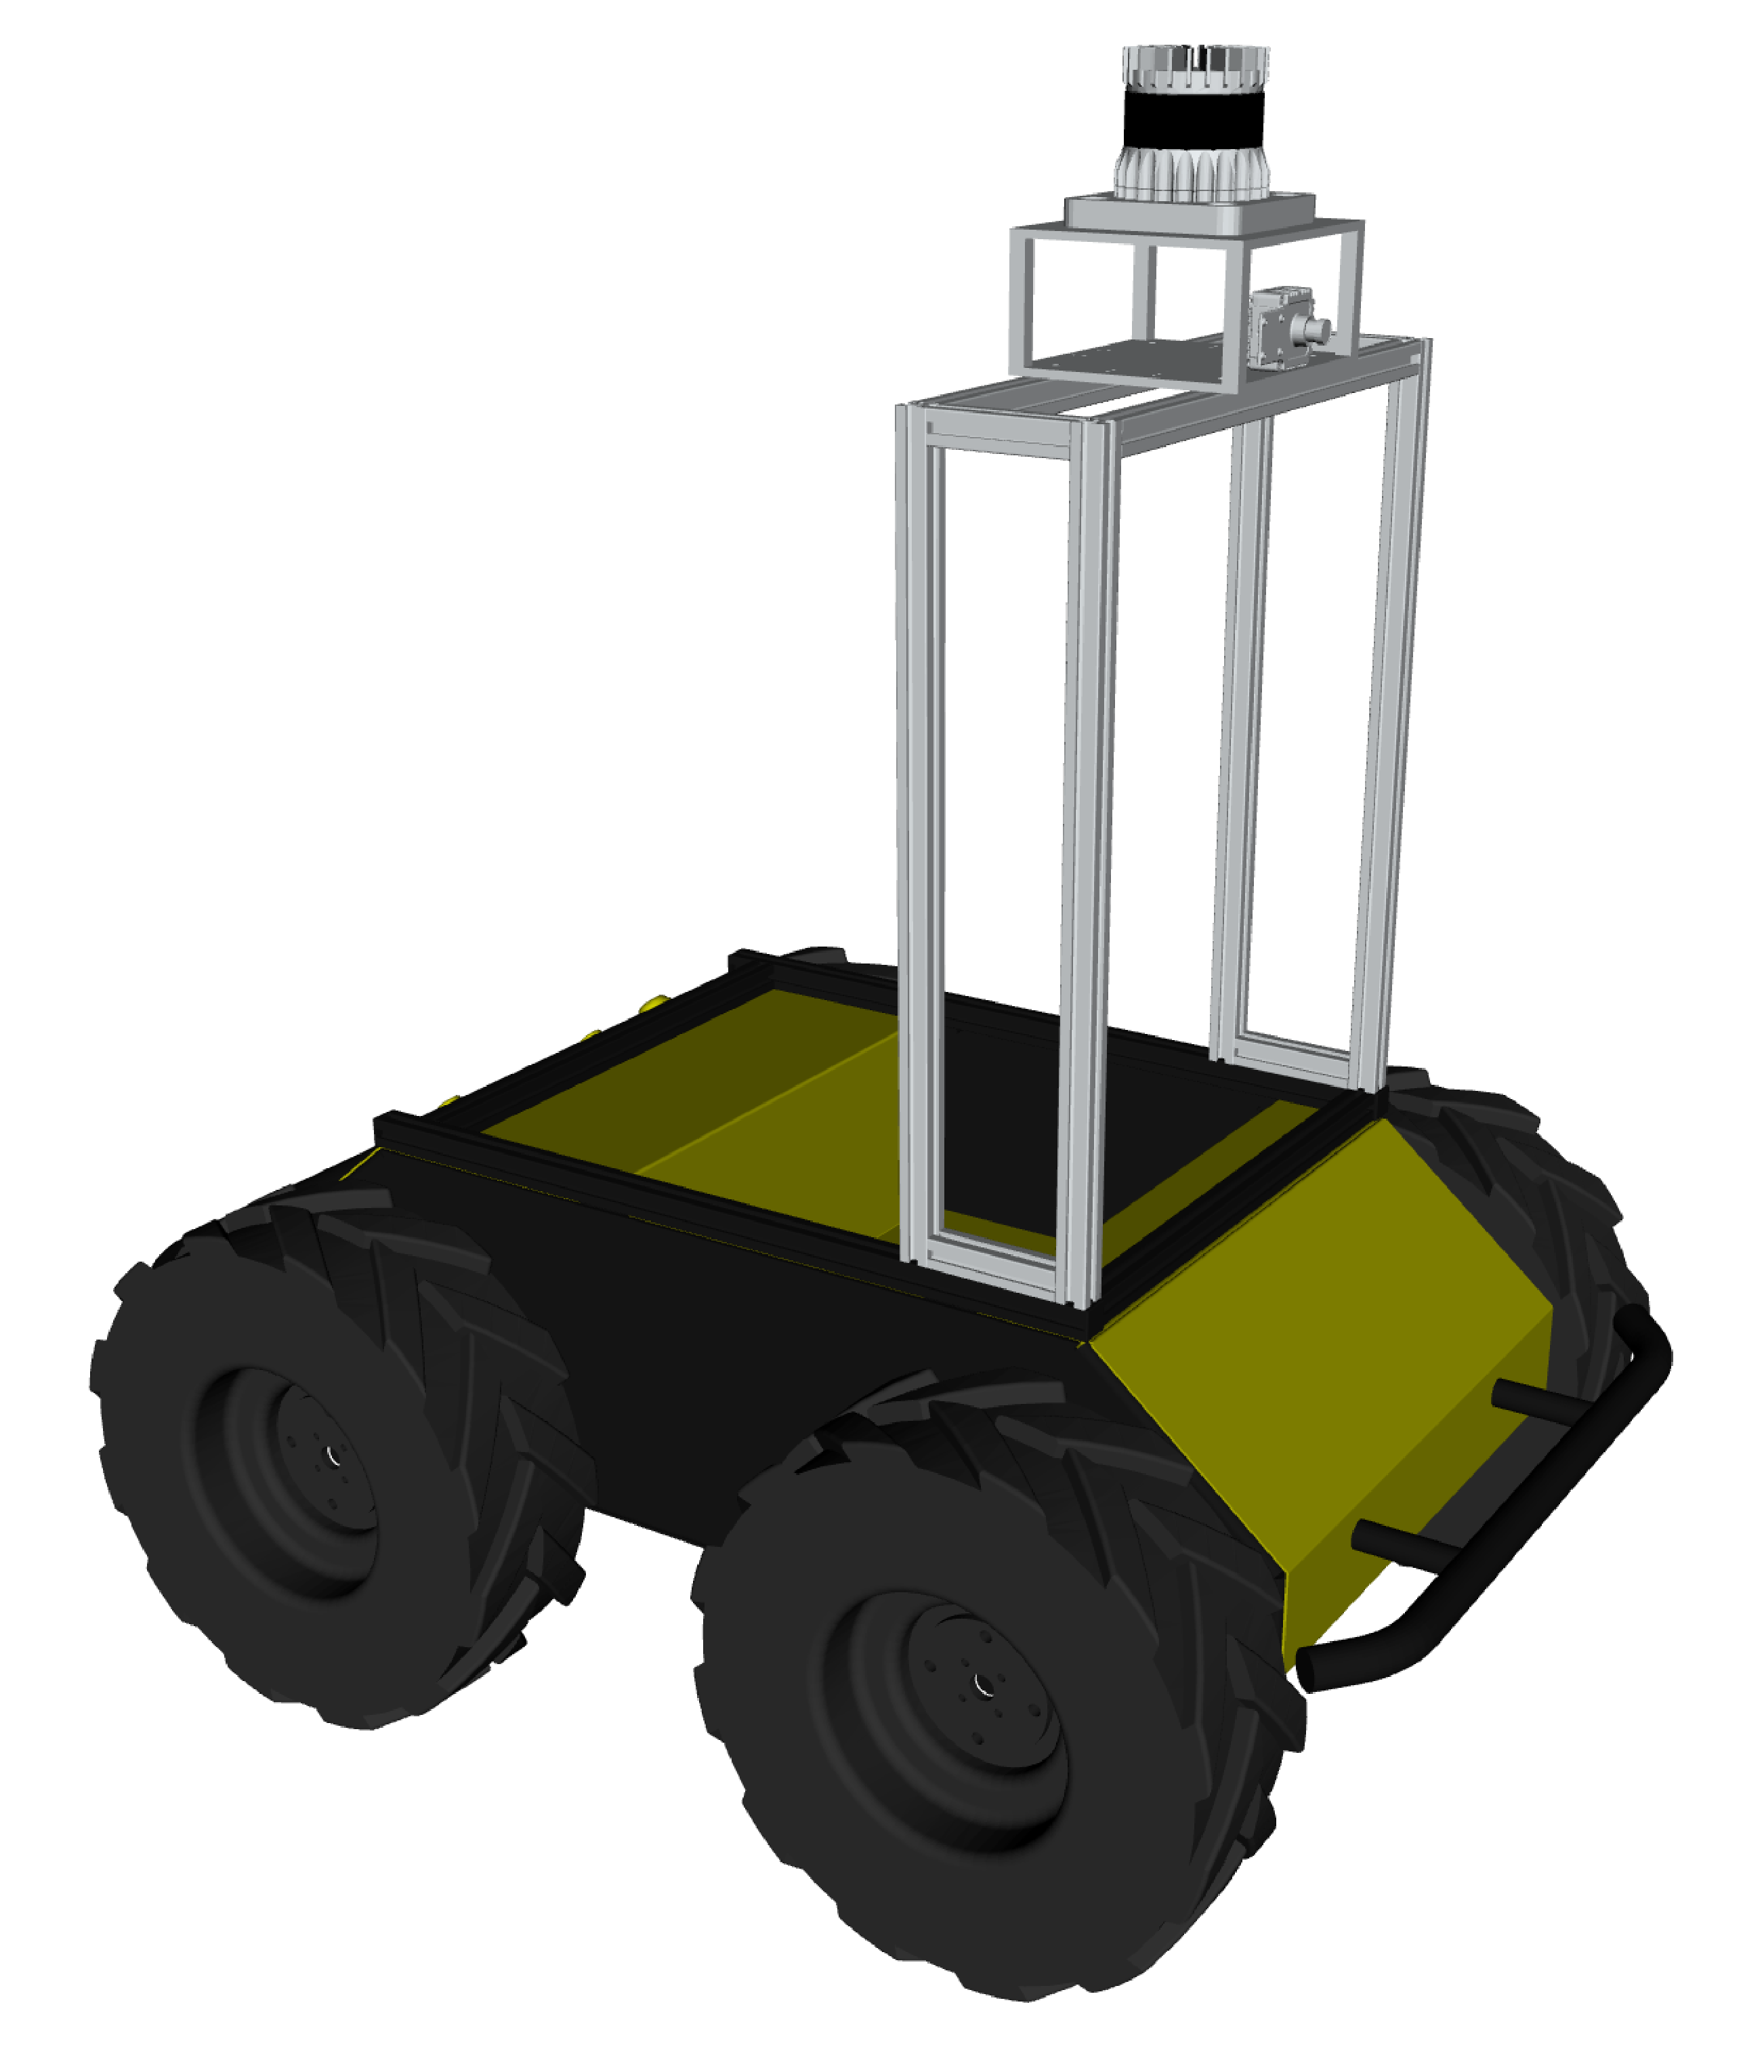
\includegraphics[width = 0.5\textwidth]{Figures/figHuskyRviz.pdf}
  \caption{Rviz2 visualisation of mobile robot running in ROS 2. This acts as a digital twin corresponding to the physical robot.}
  \label{fig:M:AN:MC:digitalTwin}
\end{figure}



% A visual representation of the UGV with all accessories attached is preferable when interacting with the robot in Rviz2. An open source library for the 3D CAD software Solidworks called "Solidworks to URDF Exporter" \cite{urdf_exporter} is used to export a CAD model of the assembly to urdf. The exporter creates a ROS compatible description package of the CAD model with transforms at user defined locations. The package itself is not used, as it is incompatible with ROS2. However, relevant urdf code and associated ".stl" mesh files is extracted and used when launching the Husky UGV.

% \subsubsection{Velocity Commands}
% The input velocity commands come from various sources such as a controller or navigation servers. These commands are published at topics to the ROS2 network. As illustrated in figure \ref{fig:rqt_teleop}, these topics are handled through the twist\_mux node. This node publishes velocity commands based on the incoming commands and the defined priority. The command is published to the \\/husky\_velocity\_controller/cmd\_vel\_unstamped topic which is used by the husky velocity controller later to process the incoming commands.

% \begin{figure}[htp]
%   \centering
%   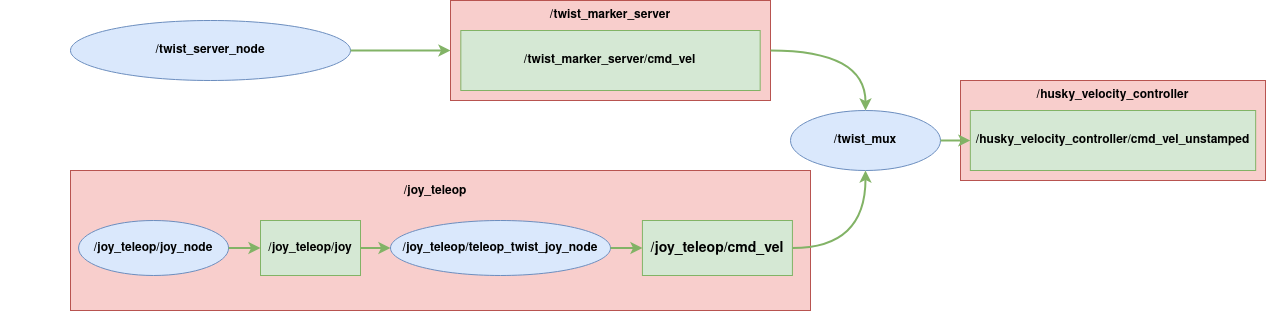
\includegraphics[width = 0.98\textwidth]{Figures/husky_teleop.drawio.png}
%   \caption{Example of how velocity commands are handled by twist\_mux node. In this example, it takes in velocity commands from the /joy\_teleop/cmd\_vel topic and the /twist\_marker\_server/cmd\_vel topic. It then forwards the velocity command based on defined priorities to the /husky\_velocity\_controller/cmd\_vel\_unstamped topic.}
%   \label{fig:rqt_teleop}
% \end{figure}
% % Aj fig not redable. increas the fontzize and make blocks compact
% \subsubsection{Controller}
% The velocity command coming from the /twist\_mux server needs to be handled by a controller in order to actuate the UGV. In the ROS2 network, this controller is represented as the husky\_velocity\_controller node. This node takes in velocity commands from the twist\_mux node, actuates the wheel motors and then calculates the motion of the UGV. The resulting odometry is published to the ROS2 topic "/odom".

\subsection{Perception}\label{sec:M:AN:Perception}
As described in section \ref{sec:M:AutonomousNavigation}, the perception system of the mobile robot consists of the Ouster OS1 LiDAR and the ROS 2 package PointCloud to LaserScan \cite{pointcloud_to_laserscan_repo}. The LiDAR provides a 3D point cloud of the environment and publishes this information to the ROS 2 network. The PointCloud to LaserScan package then converts the point cloud to a 2D laser scan that is usable by the SLAM and navigation algorithms.

The PointCloud to LaserScan package requires information about which points it should convert to laser scan. This is done by defining a maximum distance down and a maximum distance up, from the sensors origin. For example, the developer could say that all points from 1[m] below the sensor to 0.2[m] above the sensor should be considered when creating the LaserScan signal. This method takes advantage of the 3D PointCloud data set when creating a LaserScan of the surrounding area. The Resulting 2D map will therefore be valid for the whole UGV and not only for the plane where the LiDAR is located. However, since the position of the LiDAR has been altered during the course of this project, these distances has to be altered.




% However, the NAV2 navigation stack is made for 2D navigation. That is, the navigation system sets up a 2D birds eye view map of the environment and navigates this map using x, y and yaw coordinates. Therefore, the navigation system requires a 2D map.
% In order to build a 2D map of the environment, a measurement structured in 2D is needed. In ROS2, this measurement is presented in the LaserScan data type.

% \subsubsection{LiDAR Setup} \label{sec:M:MRC:LiDARSetup}
% The Ouster OS1 LiDAR provides a perception aspect to the robotic system that is used to map the surrounding environment. The LiDAR is set up with ROS2 using the ROS2 packages provided by Ouster\cite{ouster_repo}, ros2\_ouster and ouster\_msgs. The package ouster\_msgs contains definitions of data types used by ros2\_ouster. The other package, ros2\_ouster, interfaces the measurements done by the LiDAR with the ROS2 network. This way, the data can be used by other nodes on the ROS2 network.

% The LiDAR configurable with a parameter file of the type ".yaml" that can be passed to the ros2\_ouster node upon launch. Table \ref{tab:lidar_params} describes the parameters that are changed and their value compared to the default value.

% \begin{table}[H]
\centering
\caption{This table describes the LiDAR parameters that are changed for this project. Their current value and a short description of the parameter as well as their default value.}
\label{tab:lidar_params}
\vspace{1mm}
\begin{tabular}{llll}
\hline
\textbf{Parameter} & \textbf{Value}                                                        & \textbf{Description}                                                                                                           &  \\ \hline
lidar\_ip          & 169.254.171.185                                                       & \begin{tabular}[c]{@{}l@{}}IP address of LiDAR\\ \textbf{Default:} 10.5.5.96\end{tabular}                                               &  \\
computer\_ip       & 192.168.0.169                                                         & \begin{tabular}[c]{@{}l@{}}IP adress of Computer\\ \textbf{Default:} 10.5.5.1\end{tabular}                                              &  \\
sensor\_frame      & lidar\_link                                                           & \begin{tabular}[c]{@{}l@{}}TF2 base frame of sensor\\ \textbf{Default:} laser\_sensor\_frame\end{tabular}                               &  \\
laser\_frame       & base\_laser                                                           & \begin{tabular}[c]{@{}l@{}}TF2 dara frame of sensor\\ \textbf{Default:} laser\_data\_frame\end{tabular}                                 &  \\
timestamp\_mode    & \begin{tabular}[c]{@{}l@{}}TIME\_FROM\\ \_ROS\_RECEPTION\end{tabular} & \begin{tabular}[c]{@{}l@{}}Where the messages timestamp should \\ come from\\ \textbf{Default:} TIME\_FROM\_INTERNAL\_OSC\end{tabular}  &  \\
proc\_mask         & IMG|PCL|IMU                                                           & \begin{tabular}[c]{@{}l@{}}Which data that should be published to \\ the ROS2 network\\ \textbf{Default:} IMG|PCL|IMU|SCAN\end{tabular} &  \\ \hline
\end{tabular}
\end{table}

% A parameter change that is worth noticing, is the removal of "SCAN", from the parameter "\textit{proc\_mask}. This removes the LaserScan output from the LiDAR. The reason for this is that the conversion from PointCloud to LaserScan is done by another ROS2 Node. This is further explain in section \ref{sec:M:AN:Perception}.

% As mentioned earlier in section\ref{sec:M:MRC:LiDARSetup}, the LaserScan output from the Ouster OS2 LiDAR is removed. The LaserScan published by \lstinline{ros2_ouster} use the measurement from the laser that is physically oriented closest to horizontal in the LiDAR. This creates a LaserScan that measures a horizontal 2D plane around the sensor, which is how 2D $360\deg$ LiDARs usually work. However, the Husky A200 combined with all its accessories is a tall robot and having information of how a 2D plane in the environment around it looks is insufficient. Additionally, it's LiDAR provides 3D information of the environment. Therefore, the ROS2 package \lstinline{pointcloud_to_laserscan} takes care of the conversion from PointCloud to LaserScan. 


\subsection{Localisation and Mapping} \label{sec:M:AN:LocalisationAndMapping}
The localisation and mapping system seen in figure \ref{fig:M:AN:ANMethod}, is a combination of several subsystems, mainly an EKF filter and a SLAM algorithm. The UM7 IMU can also be seen in \ref{fig:M:AN:ANMethod} as a part of this system as it's data is only used for localisation. A bloated figure further explaining localisation and mapping is shown in figure \ref{fig:M:AN:LAM:LocMapping}.

\begin{figure}[htp]
    \fontsize{8}{10}\selectfont
    \centering
    \includesvg[width = 1\textwidth]{Figures/figLocMapping.drawio.svg}
    \caption{Localisation and mapping}
    \label{fig:M:AN:LAM:LocMapping}
\end{figure}


\subsubsection{IMU Setup} 
To be able to use the UM7 IMU with ROS2, it has to be set up as a ROS2 node. This is done by using UM7 ROS2 packages provided by \cite{um7_repo}. This node sets a connection to the UM7 IMU through USB and publishes measurements to the ROS topic "/imu/data". The node is dependent on \cite{serial_repo} which is a library for interfacing with serial communication.


 \subsubsection{Extended Kalman Filter}
In order to more accurately calculate the movement of the UGV, an extended kalman filter is use. The ekf filter fuses UGV odometry with IMU data from both the UM7 IMU and OS1 LiDAR's built in IMU. Figure \ref{fig:rqt_ekf} illustrates how the extended kalman filter(ekf\_node) takes in odometry data from the UGV(husky\_velocity\_controller) as well as IMU data from the UM7 IMU(um7\_driver) and the OS1 LiDAR(ouster\_driver). The node ekf\_node then fuses the odometry and IMU data in order to calculate the transform from /odom to /base\_link.

\begin{figure}[htp]
  \centering
  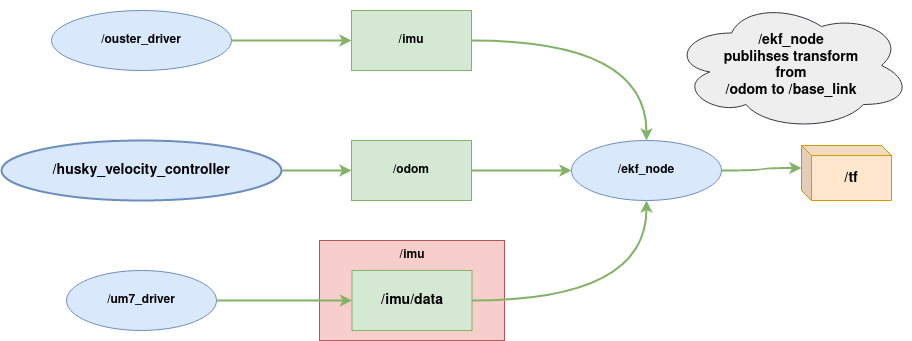
\includegraphics[width = 1\textwidth]{Figures/husky_nodess.drawio.png}
  \caption{Illustration of how the ekf\_node fuses the odometry from the husky\_velocity\_controller and IMU data from both the ouster\_driver and the um7\_driver.}
  \label{fig:rqt_ekf}
\end{figure}

\subsubsection{Simultaneous Localisation And Mapping}
Simultaneous localisation and mapping (SLAM) is used to give a final robot pose estimate along with a map. The SLAM algorithm itself is provided by the ROS2 package SLAM Toolbox. The ROS2 node takes in odometry information from the motion control system together with LaserScan from the perception system to localise and generate a 2D map of the environment. Because of the use of "PointCloud to LaserScan", the resulting map contains all obstacles in the "collision zone" of the mobile robot. Obstacles that are too low to be mapped can be traversed by the mobile robot and obstacles that are located too high will be ignored. When looking at localisation, there are several methods that could be used. As SLAM is already used for mapping, it becomes a natural choice for preforming the localisation task as well. SLAM Toolbox utilises a pose-graph approach to the SLAM problem, based on the SPA technique mentioned in section \ref{sec:T:AN:L:SLAM}.

% Since SLAM algorithms does both mapping and localisation simultaneously, it gives an accurate representation of an environment for navigation and places the robot in this environment. Therefore, SLAM toolbox is used alongside NAV2 during autonomous navigation. 

\subsection{Navigation}
As the UGV platform is set up with compatible motion control, perception, mapping and localisation systems, it is now able to run the ROS2 Navigation stack NAV2. This is the standard autonomous navigation library for mobile robots in ROS2. In ROS2 Galactic, NAV2 introduced a simple API towards Python, which is used by a custom Top Level ROS2 node to interact with NAV2. The Top Level node is described later in section \ref{M:TopLevel}. Since this API is introduced in Galactic, the choice was made to use ROS2 Galactic for NAV2. This means that SLAM Toolbox also has to run in ROS2 Galactic to ensure compatibility between the two.

As long as the other systems are up and running, the navigation stack should be ready for use. However, there is a parameter \lstinline{.yaml} file that could require tweaking in order to achieve optimal performance. By default, the file is set up to fit smaller mobile robots. As the mobile robot in this project is quite large, adjustments to the inflation layer of the navigational maps has been made. The inflation layers tells the navigational system how close the robot is allowed to get to obstacles in the map. Another adjustment regards the footprint of the robot. The robot footprint in NAV2 defines the outline of the mobile robot relative to it's origin. Footprint adjustment is done by Didrik Robsrud as a part of the work on his thesis on Radar-LiDAR sensor fusion in ROS. Lastly, the moving window that defines the size of the local planner(obstacle avoidance), is increased to better fit the larger dimensions of the mobile robot

\section{Pick and Place} \label{M:PickAndPlace}

\begin{figure}[htp]
  \centering
  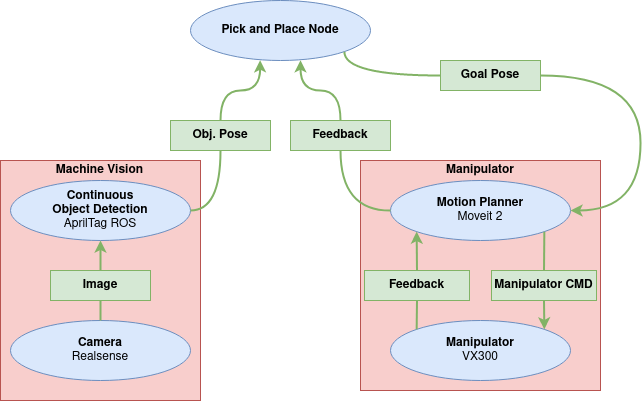
\includegraphics[width = 0.98\textwidth]{Figures/figPickAndPlaceMethod.drawio.png}
  \caption{This figure illustrates the Pick and Place subsystem}
  \label{fig:M:PAP:PickAndPlaceMethod}
\end{figure}

\subsection{Machine Vision} \label{sec:M:MRC:MachineVision}
The machine vision system is comprised by an Intel Realsense D435i, as described in section \ref{sec:M:H:P&PH:ManipulatorMountedCamera}, and an AprilTag based 6-DOF pose estimation system described in section \ref{sec:M:MRC:MV:TagDetectionSystem}. This creates at robust machine vision system that achieves what is observed as real-time pose estimation.

\subsubsection{Vision Camera} 
The gripper mounted Realsense camera provides flexible machine vision wherever the manipulators gripper is pointing. Intel provides ROS2 packages for Realsense cameras that interfaces with the ROS2 network \cite{realsense_ros_repo}. These packages publishes data from the Realsense camera to the ROS2 network so that it is available for other nodes on the network. The ROS2 Realsense packages requires Intel RealSense SDK 2.0 which is available as debian packages for AMD Ubuntu machines. For Xaviers, whom are running an ARM architecture, the SDK is available to be built from source on Github\cite{realsense_jetson_guide}.

\subsubsection{Tag Detection System} \label{sec:M:MRC:MV:TagDetectionSystem}
The AprilTag based detection system is set up using the open source packages provided by \cite{apriltag_repo}, \cite{apriltag_ros_repo} and \cite{apriltag_msgs_repo}. These packages are used to create a ROS2 node that will run continuous AprilTag detection on the defined camera stream. Section \ref{sec:T:OD:TagBasedObjectDetection} mentions tag families, which is collections of pre-defined AprilTags for use by developers. In this project, the standard tag family "\textit{tag36h11}" is used. The AprilTag ROS2 node requires the tags of the chosen tag family to be defined in a \textit{".yaml"} parameter file. The parameter file describes the name and physical size of each tag, which is vital information for this kind of machine vision system. An example of a tag definition can be seen in listing \ref{lst:M:M:MachineVision}.

\begin{lstlisting}[language=XML, label=lst:M:M:MachineVision, caption={Example of AprilTag tag definitions in a ".yaml" file. This example defines two tags of different names, using the tag id 0 and 1 in the defined tag family The size is alse defined for each tag. The tag family (tag36h11) is set in another parameter file.}]
/**:
  ros__parameters:
    standalone_tags:
      tag_names: ["my_tag_0", "my_tag_1"]
      my_tag_0:
        id: 0
        size: 0.135
      my_tag_1:
        id: 1
        size: 0.0344
\end{lstlisting}

In listing \ref{lst:M:M:MachineVision}, the tags \lstinline{my_tag_0} and \lstinline{my_tag_1} are defined. The "id" parameter on each tag definition links this definition to a specific AprilTag in the AprilTag family \textit{"tag36h11"}. It is mentioned in the previous paragraph that the node runs continuous detection. This means that the node will continuously look for AprilTags in the camera stream for as long as it is running. When the AprilTag node detects an AprilTag, it will check if the detected tag is defined in the parameter "\textit{.yaml}" file. If so, it will use the defined size together with the information in the camera stream to publish a 6-DOF pose of the tag to the ROS2 network. The published pose will be on the form of a TF2 transform with the same name as the tag (ex. \lstinline{my_tag_0}).

\subsection{Manipulator}\label{sec:M:MRC:Manipulator}
Interbotix provides ROS2 packages for the VX300 manipulator. The most relevant of these being the package \lstinline{interbotix_xsarm_moveit}, which is used to bring up the VX300 manipulator in Moveit2 for motion planning and control of the arm as well as Rviz2 with a GUI for running and testing the Moveit2 configuration. Figure \ref{fig:VX300Moveit} illustrates a virtual VX300 manipulator running with Moveit2 and visualised in Rviz2. The Moveit2 Motion Planning GUI is located in the lower left corner of the figure. The actual manipulator pose is illustrated by a black manipulator and the goal pose is illustrated by an orange manipulator. In figure \ref{fig:VX300Moveit}, the manipulator is oriented at the goal pose. The orange goal pose shines through the actual pose at the fingers.

\begin{figure}[htp]
  \centering
  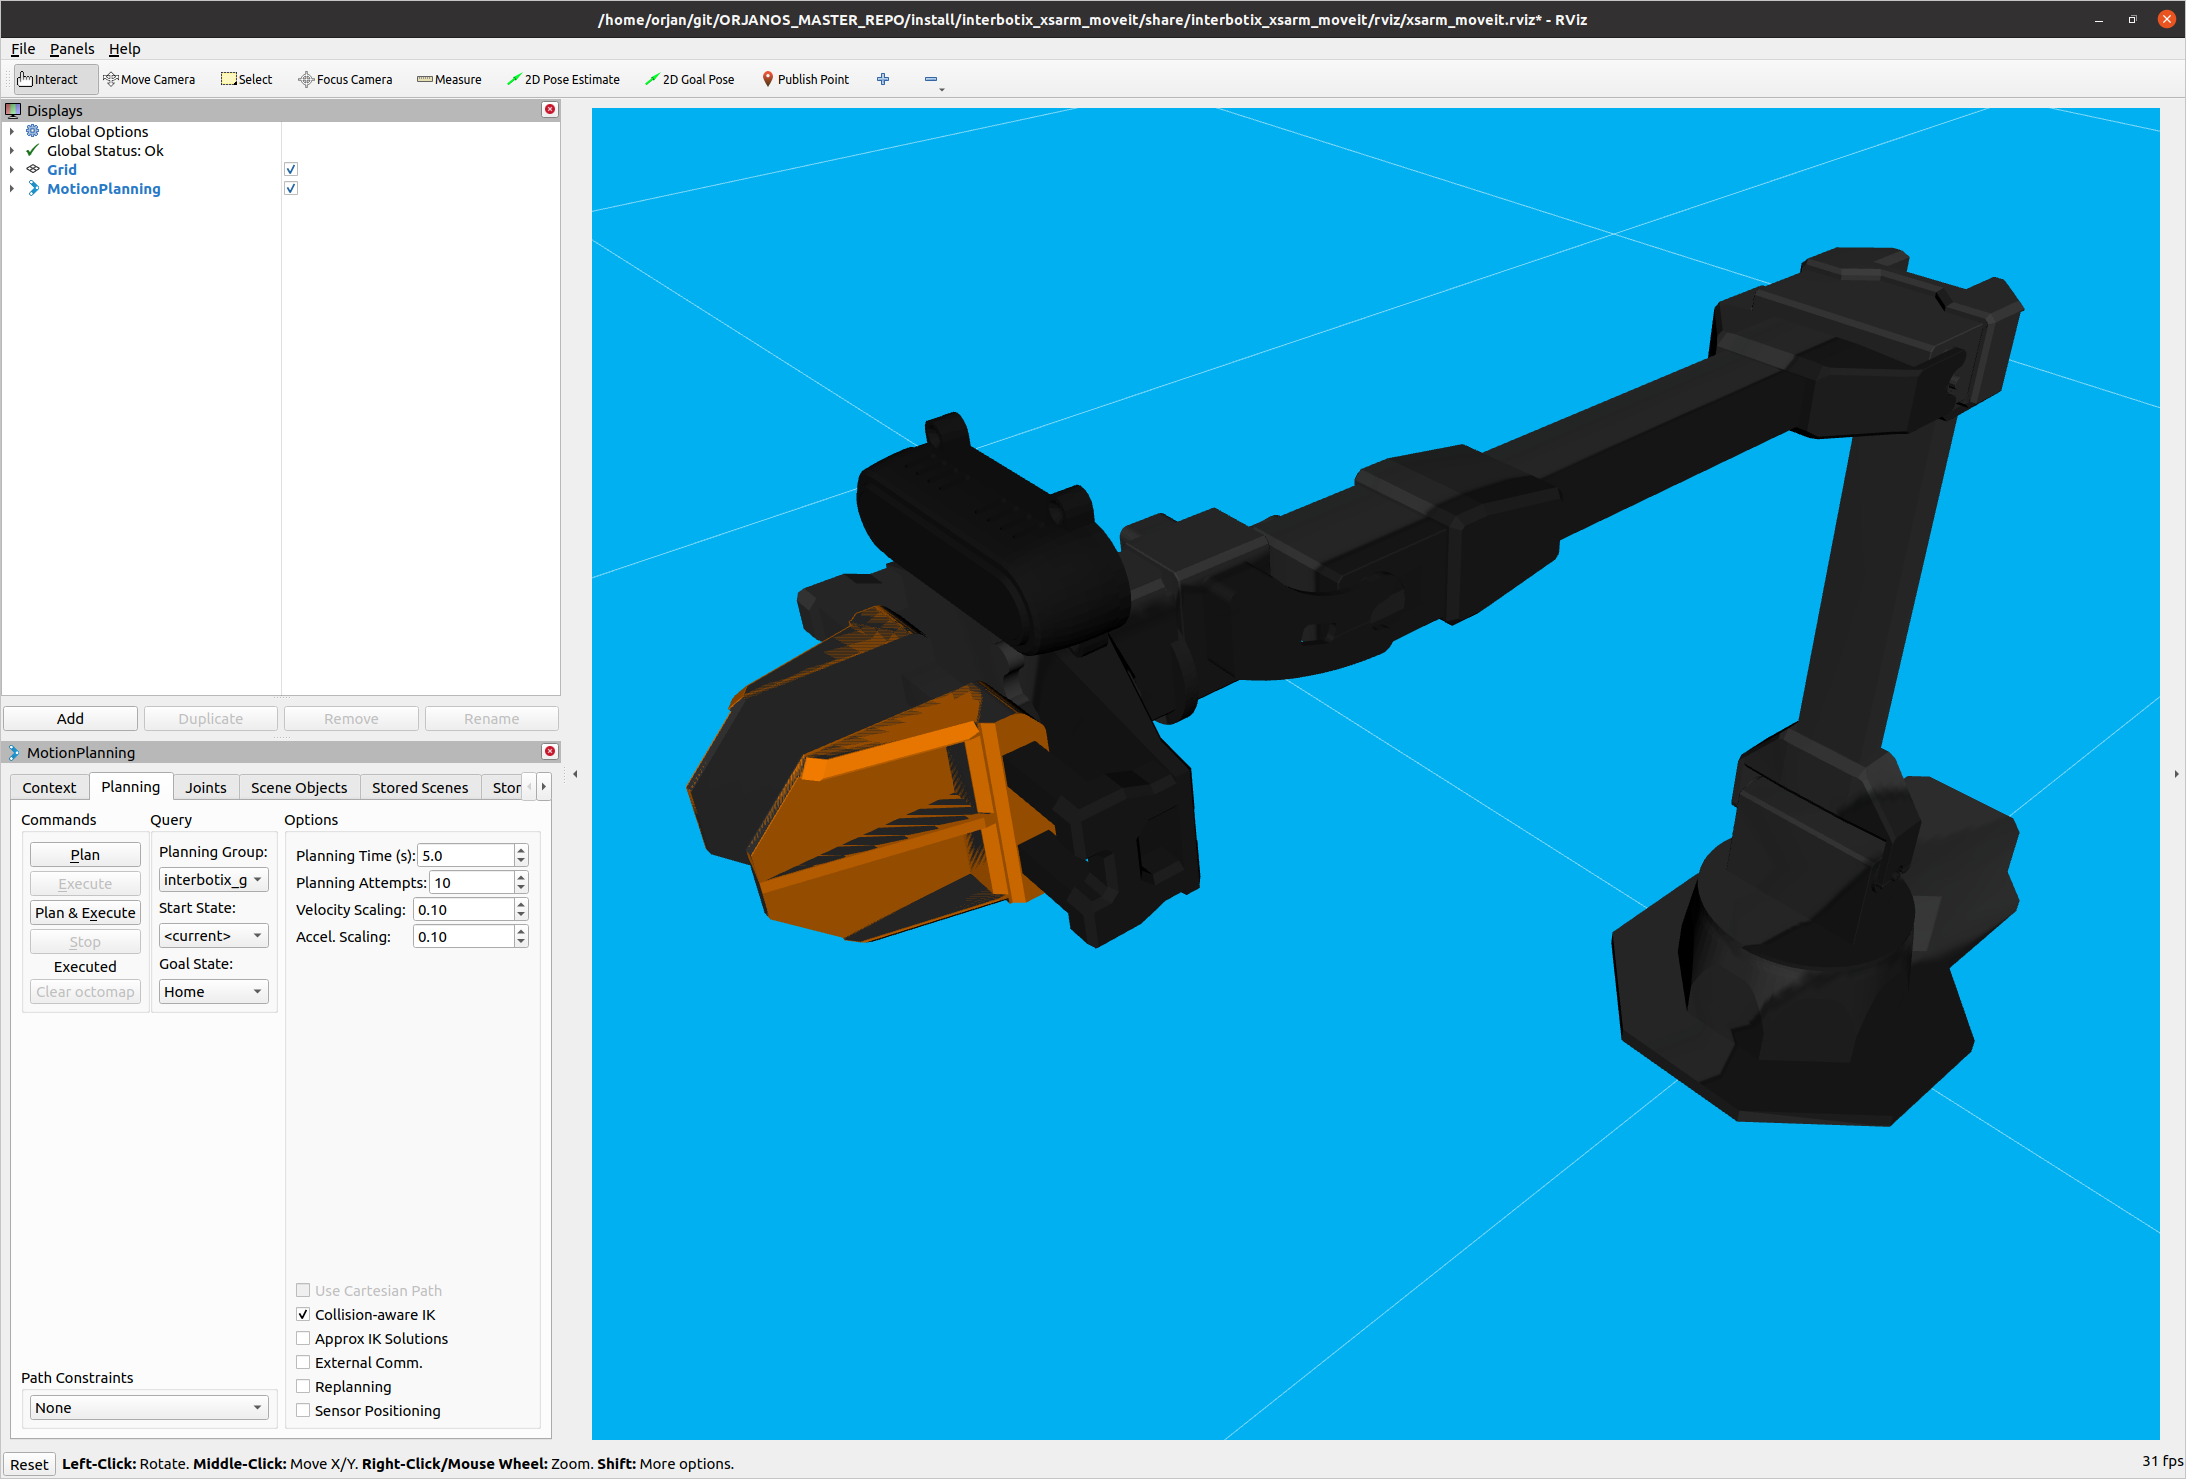
\includegraphics[width = 1\textwidth]{Figures/figVX300Moveit.png}
  \caption{A virtual VX300 manipulator running Moveit2 and visualised in Rviz2. The Moveit2 Motion Planning GUI is located in the lower left corner of the figure. The actual manipulator pose is illustrated by a black manipulator and the goal pose is illustrated by an orange manipulator which shines through at the gripper fingers. The Realsense camera can be seen mounted on top of the gripper.}
  \label{fig:VX300Moveit}
\end{figure}

\subsubsection{Model Description}
Looking at figure \ref{fig:VX300Moveit}, it can be seen that the Realsense camera, described in section \ref{sec:M:H:PickandPlaceHardware}, is mounted on top of the VX300 gripper using its mounting bracket. This is practical for visualisation, but also necessary to avoid collisions with both surrounding objects, and the manipulator itself. Similarly to how accessories were added to the UGV in section \ref{sec:M:CS:UGV:S:ModelDescription}, the Realsense camera assembly is generated through the open source urdf exporter\cite{urdf_exporter}. 

\subsubsection{Planning Scene}
In Moveit2, the planning scene describes the environment around the manipulator. Objects and barriers described in the planning scene will be taken into account by the planner when planning a manipulator motion. As this manipulator is mounted on top of the mobile robot, the manipulator needs to have a perspective of the shape and position of the mobile robot in order to avoid collision. As mentioned in section \ref{sec:M:CD:InitialConcept}, the mobile robot is running on the "UGV Xavier", and the manipulator is running on the "Manipulator Xavier". Both these robotic devices are described by xacro files on the form of urdf. However, they take in pure urdf files for accessories. This means that there is no easy way to add the urdf file of one as an accessory to the other. As a result, the robotic description of the mobile robot and the manipulator is separated. To take the mobile robot into account when planning manipulator motion, the shape of the husky is therefore added to the planning scene in Moveit2 as collision boxes.

In the Motion planning GUI seen in the lower left corner of figure \ref{fig:VX300Moveit}, collision boxed can be added to the planning scene through the "Scene Objects" tab. This is a simple interface where it is possible to add different geometric shapes with a defined size and position. After defining a planning scene, the scene can be exported to a ".scene" file which can be used later to import the same scene. In this project, a ROS2 node that parses ".scene" files and publishes the information in them to the manipulator's planning scene is developed.

\subsubsection{Scene Geometry Publisher} \label{sec:M:PAP:SceneGeometryPublisher}
As mentioned in the previous paragraph, a ROS2 node that parses a "\textit{.scene}" file and publishes the information in this file to the planning scene is developed. This node consists of a custom C++ Class, the implementation of this class, a launch file and a "scene" folder to put \textit{.scene} files. An UML class representation of the ScenePublisher C++ class can be seen in figure \ref{fig:scenePublisherUML}.

\begin{figure}[htp]
  \centering
  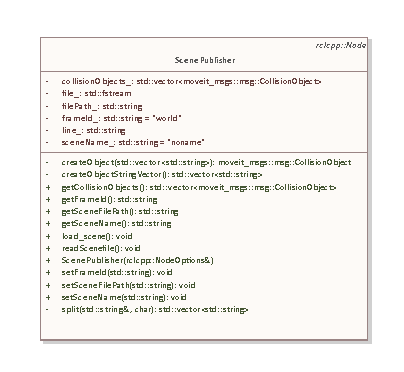
\includegraphics[width = 0.8\textwidth]{Figures/scene_geometry_publisher.pdf}
  \caption{UML Class Diagram of the Scene Geometry publisher Node.}
  \label{fig:scenePublisherUML}
\end{figure}

It can be seen from figure \ref{fig:scenePublisherUML} that ScenePublisher inherits from "rclcpp::Node".  Ros Client Library for C++(RCLCPP) is the official C++ API towards for interacting with ROS2. Inheriting from  "rclcpp::Node" means that ScenePublisher will have all the functionality of a standard C++ ROS node in addition to the functionality added to it. When an instance of a ScenePublisher is initiated, it will run the constructor \lstinline{ScenePublisher(rclcpp::NodeOptions&)}, which sets the scene file path to the default path (.scene file in scene folder of the package). The constructor requires an \lstinline{rclcpp::NodeOptions} variable where the developer is able to pass custom options to the node. Algorithm \ref{alg:M:ScenePubImplement} describes how the \lstinline{ScenePublisher} class is implemented in the Scene Geometry Publisher node.

\begin{algorithm}[htp!]
    \caption{Implementation of scene publisher class.} \label{alg:M:ScenePubImplement}
    \begin{algorithmic}[1] 
            \State $jointStateTopic \gets "vx300/joint\_states"$ \Comment{Declare param override}
            \State $opt \gets nodeOptions(jointStateTopic)$ \Comment{Declare options with custom param}
            \State $node \gets ScenePublisher(opt)$\Comment{Init ScenePublisher class with param override}
            \State $node.setSceneFilePath(sceneFilePath)$ \Comment{Set scene file path if alternative path is wanted}
            \State $node.readSceneFile()$ \Comment{Read .scene file, store in $file\_$}
            \State $node.loadScene()$ \Comment{$loadScene()$ described in alg. \ref{alg:M:scenePubLoadScene}}
            \State $PlanningSceneInterface \;\; planningSceneInterface$ \Comment{Declare planning scene interface}
            \State $planningSceneInterface.apply(node.getCollisionObjects())$\Comment{Publish Collision objects using interface}
            \State \textbf{shutdown}           
    \end{algorithmic}
 \end{algorithm}

After initiation of a ScenePublisher node, the ".scene" file path ca be changed using the \lstinline{setSceneFilePath()} method (line 3 in alg \ref{alg:M:ScenePubImplement}). Furthermore, \lstinline{readSceneFile()} (line 4 in alg \ref{alg:M:ScenePubImplement}) should be used to read the specified ".scene" file and store its information in a member variables of the class. After this, the method \lstinline{loadScene()} (line 5 in alg \ref{alg:M:ScenePubImplement}) is used to parse the information from the ".scene" file into a vector of collision objects that are stored a member variable of the class. Algorithm \ref{alg:M:scenePubLoadScene} describes \lstinline{loadScene()} in more detail later. 

\begin{algorithm}[htp!]
    \caption{Algorithm describing how scenes are loaded into collision objects with $loadScene()$ method.} \label{alg:M:scenePubLoadScene}
    \begin{algorithmic}[1]
            \State $getline(file\_,line\_)$ \Comment{Reads line from $file\_$, stores in $line\_$}
            \State $sceneName \gets line\_$ \Comment{First line is scene name}
            \State $getline(file\_,line\_)$
            \State $token \gets split(line\_,"\;")$ \Comment{Split line at spaces, store in "token" vector}
            \While{$token[0] == "*"$} \Comment{"*" Denotes beginning of new object}
                \State $objectStringVector \gets createObjectStringVector()$ \Comment{Parse object info}
                \State $collisionObject \gets createObject(ObjectStringVector)$ \Comment{Create collisionObject from info}
                \State $collisionObjects.push\_back(collisionObject)$ \Comment{Store collisionObject in vector/array}
                \State $token \gets split(line\_,"\;")$
            \EndWhile
            \State $collisionObjects\_ \gets collisionObjects$ \Comment{Store in class member variable}
    \end{algorithmic}
 \end{algorithm}

 

As all information in the ".scene" file is extracted using \lstinline{readSceneFile()}, it can be accessed using \lstinline{getLine()}. The first line in a ".scene" file is always the scene name. This is stored in a member variable of the class (line 2 in alg \ref{alg:M:scenePubLoadScene}). The while loop at line 5-10 in algorithm \ref{alg:M:scenePubLoadScene} will read the rest of the file and store the parsed information into a vector of collision objects. Looking at the contents of this wile-loop, \lstinline{createObjectStringVector()} will write the contents of one object and store it in a string (line 6 in alg \ref{alg:M:scenePubLoadScene}). This string will be passed into \lstinline{createObject()} which creates the corresponding collision object and stores this in a collision object variable (line 7 in alg \ref{alg:M:scenePubLoadScene}). This object is then added to the end of a vector of collision objects (line 8 in alg \ref{alg:M:scenePubLoadScene}). The loop is run until there are no more objects in the file. After parsing is done, the collision objects is stored in a member variable of the class. After all collision objects have been parsed and stored, an interface towards the planning scene is initiated (line 6 in alg \ref{alg:M:ScenePubImplement}) and the collision objects are applied to the scene (line 6 in alg \ref{alg:M:ScenePubImplement}).


% It can also be seen that \lstinline{frameID_} is hard coded to "\textit{world}", the default base link of Interbotix manipulators.

\subsubsection{Pick and Place Package} \label{sec:M:A:HuskyPickAndPlace}
In order to easier interact with Moveit2, a custom "Pick and Place" package is developed. This node listens for incoming commands through the custom ROS2 topic \lstinline{/action} and provides feedback about its operating status on the custom ROS2 topic \lstinline{/action_status}. Based on the incoming commands, the node will preform different pick and place related operations with the Interbotix VX300 manipulator. The manipulator is limited to 5 degrees of freedom. This restricts the manipulators ability to reach certain positions. Therefore, the target poses has to take this into account. This problem is most prevalent when picking, as the target object could have any pose.
The chosen solution is to always pick the target objects from the top. This solution places the following restrictions on the system in that object rotation around x-axis, $\rho$, and y-axis, $\theta$, is neglected. The object is then assumed to be placed on a level surface. Only xyz-position and z-rot will be taken into account when picking the object. 
The package consists of a C++ class and the implementation of this class. As with the scene publisher, an UML class diagram of the C++ class is made to better illustrate the contents of the class. The diagram can be seen in figure \ref{fig:PickAndPlaceUML}.

\begin{figure}[htp]
  \centering
  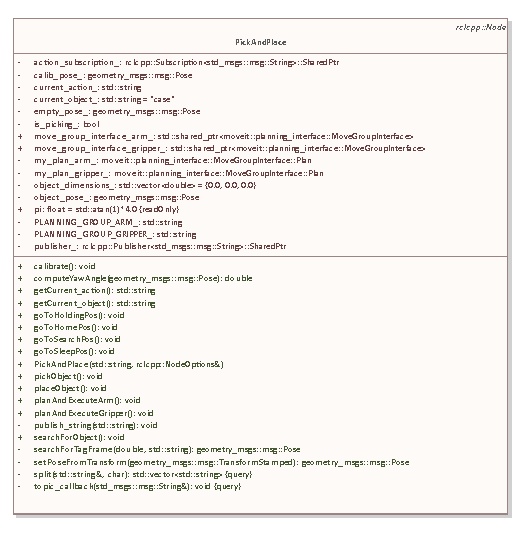
\includegraphics[width = 0.8\textwidth]{Figures/husky_pick_and_place.pdf}
  \caption{UML Class Diagram of the Husky Pick and Place Node.}
  \label{fig:PickAndPlaceUML}
\end{figure}

Looking at figure \ref{fig:PickAndPlaceUML}, it can be seen that the PickAndPlace C++ class inherits from the same \lstinline{rclcpp::Node} as the ScenePublisher class. Upon initiation of the PickAndPlace Class, the constructor \lstinline{PickAndPlace(std::string move_group_namespace, rclcpp::NodeOptions&)} will be called. This constructor requires two variables. A namespace definition, corresponding to the defined manipulator name and an \lstinline{rlccpp::NodeOptions} variable. The Options variable is used to give the developer possibilities to pass custom variables to the node, as with the ScenePublisher class.
The constructor will set up a subscription to the \lstinline{/action} topic and a publisher to the \lstinline{/action_status} topic. The subscription will constantly listen for messages on the \lstinline{/action} topic and store any messages it detects in the member variable \lstinline{action_subscription_} seen in figure \ref{fig:PickAndPlaceUML}. The Publisher will be used by class methods to publish status feedback to the \lstinline{\action_status} topic.

Algorithm \ref{alg:M:PaPImplement}, describes how the Pick and Place class is implemented and used in the ROS2 node \lstinline{pick_and_place}. As it can be seen from this algorithm, the implementation of the class is quite simple. The first two lines involves setting a parameter and initiating the ROS2 node. The main functionality is gathered in one while-loop. Looking closer at that while-loop, it can be seen that the $getCurrentAction()$ function is called in every if-condition This function  returns a string containing the last message the node got through the \lstinline{/action} topic . If the data on the "\lstinline{/action}" topic fits one of the if-conditions, the corresponding operation is preformed.

\begin{algorithm}[htp]
    \caption{Algorithm describing how the Pick and Place class is implemented} \label{alg:M:HuskyMaster}
    \begin{algorithmic}[1] 
            \State $manipulatorNamespace \gets "vx300"$ \Comment{Declare namespace}
            \State $opt \gets NodeOptions()$ \Comment{Declate node options}
            \State $node \gets PickAndPlace(manipulatorNamespace, opt)$\Comment{Init PickAndPlace class with namespace and opt}
            \While{\textbf{not} ERROR}
                \If{$node.getCurrentAction() == "pick"$}
                    \State $node.goToSearchPos()$
                    \State $node.searchForObject()$
                    \State $node.pickObject()$
                \ElsIf{$node.getCurrentAction() == "place"$}
                    \State $node.placeObject()$
                \ElsIf{$node.getCurrent\_action() == "calibrate"$}
                    \State $node.calibrate()$
                \ElsIf{$node.getCurrent\_action() == "sleep"$}
                    \State $node.goToSleepPos()$
                \EndIf
            \EndWhile
            \State \textbf{shutdown}         
    \end{algorithmic}
 \end{algorithm}

Looking at algorithm \ref{alg:M:PaPImplement}, \textit{searchForObject()} is called in line 6. This function will search for a specified object coordinate frame and store it's pose in an \textit{objectPose\_} variable. The object's coordinate frame will b provided by the machine vision package if there are any objects available. Algorithm \ref{alg:M:PaPSearch} describes how \textit{searchForObject()} is implemented.

\begin{algorithm}[htp!]
    \caption{Algorithm describing how Object Detection and pose est. is preformed in the Pick and Place Package} \label{alg:M:PaPSearch}
    \begin{algorithmic}[1]
        \renewcommand{\algorithmicrequire}{\textbf{Input:}}
       \renewcommand{\algorithmicensure}{\textbf{Output:}}
       \Require $(timeout \gets 10.0s)$, $(tag\_frame \gets "")$
       \Ensure $pose$
            \State $frameAvailable \gets$ \textbf{false}
            \If{$tagFrame == ""$} \Comment{Set $tagFrame$ to default if not set}
                \State $tagFrame \gets currentObject\_ + "\_tag"$
            \EndIf
            \State $startTime \gets clockNow$
            \While{(\textbf{not} ERROR) \textbf{and} (\textbf{not} $frameAvailable$)}
                \try
                    \State $transform \gets lookupTransform(planning\_frame, pose\_frame)$
                    \State $frame\_available \gets$ \textbf{true}
                \catch{Frame not Found}
                    \State sleep for 100 milliseconds \Comment{Frame not available yet, wait and try again}
                \endtry
                \State $elapsedTime \gets clockNow - startTime$
                \If{$elapsedTime \geq timeout$}
                    \State Throw ERROR("Timeout reached while looking for tag!")
                    \State \Return $emptyPose$
                \EndIf
            \EndWhile
            \If{\textbf{not} $frameAvailable$}
                \State \Return $emptyPose$
            \EndIf
            \State $pose \gets setPoseFromTransform(transform)$ \Comment{Convert to correct datatype}
            \State \Return $pose$
    \end{algorithmic}
 \end{algorithm}

After search has been preformed using \ref{alg:M:PaPSearch} the object can be picked. This is done using the \lstinline{pickObject()}  method. This method will start by moving the gripper above the detected object to take a new measurement of the objects pose with the machine vision system. Then, the manipulator will pick the object based on the updated measurements and hold it in a "holding pose". This holding pose is suitable for holding objects while the Autonomous Navigation system navigates to another location. The \lstinline{pickObject()}  method is described in more depth in algorithm \ref{alg:M:PaPPick}. 

\begin{algorithm}[htp!]
    \caption{Algorithm describing object Picking is Preformed, using $pickObject()$ method} \label{alg:M:PaPPick}
    \begin{algorithmic}[1]
            \State publishString("picking") \Comment{Feedback to Top Level System}
            \State $currentAction\_ \gets "none"$ \Comment{Reset command from "/action" topic}
            \If{$objectPose_ == emptyPose$}
                \State Throw ERROR("No object pose stored, aborting picking procedure!")
                \State Throw EROOR("Run 'searchForObject()' to populate the objectPose\_ variable!")
                \State Plan and execute move to sleepPose
                \State \textbf{return}
            \EndIf
            \State $objectPose \gets objectPose\_$ \Comment{Get pose from member var}
            \State $[x, y, z] \gets getXYZ(objectPose)$ \Comment{Extract XYZ}
            \State $[\rho, \theta, \phi] \gets getRPY(objectPose)$ \Comment{Extract RPY as $[\rho, \theta, \phi]$}
            \State $denum \gets x$ 
            \If{$denum == 0$}
                \State $denum \gets 0.000001;$
            \EndIf
            \State $qYaw \gets \arctan\left ( \frac{y}{denum}\right )$ \Comment{same as: $qYaw \gets computeYawAngle(objectPose\_)$}
            \State $heightAbove \gets 0.3m$ \Comment{Inspection height above object}
            \State $shift \gets 0.0m$ \Comment{Brings Gripper closer in xy-coords to base}
            \State $xInsp \gets x - shift\cdot \cos(qYaw)$
            \State $yInsp \gets y - shift \cdot \sin(qYaw)$
            \State $zInsp \gets z + heightAbove$
            \State $poseInsp.Pos \gets setXYZ(xInsp, yInsp, zInsp)$
            \State $poseInsp.Orient \gets setRPY(0, \frac{\pi}{2}, \phi)$ \Comment{5-DOF arm: using only $\phi$}
            \State Plan and execute move to poseInsp \Comment{Directly above object, looking down at it}
            \State Plan and execute gripper released
            \State $searchForObject()$ \Comment{To get a better pose estimate, do a new measurement}
            \State $objectPose \gets objectPose\_$ \Comment{Get pose from member var}
            \State $[x, y, z] \gets getXYZ(objectPose)$ \Comment{Extract XYZ}
            \State $[\rho, \theta, \phi] \gets getRPY(objectPose)$ \Comment{Extract RPY as $[\rho, \theta, \phi]$}
            \State $poseAboveObj.Pos \gets setXYZ(x, y, z+0.05)$
            \State $poseAboveObj.Orient \gets setRPY(0, \frac{\pi}{2}, \phi)$ \Comment{5-DOF arm: using only $\phi$}
            \State Plan and execute move to poseAboveObj \Comment{Moves to 0.05m above objectPose}
            \State $poseAtObj.Pos \gets objectPose.Pos$
            \State $poseAtObj.Orient \gets poseAboveObj.Orient$ \Comment{5-DOF arm: using only $\phi$}
            \State Plan and execute move to poseAtObj
            \State $poseGripperGrasp \gets "Grasping\_" + currenObject\_$ \Comment{Grasping pose defined in srdf file}
            \State Plan and execute poseGripperGrasp
            \State $poseLiftObj.Pos \gets setXYZ(x, y, z+0.2)$
            \State $poseLiftObj.Orient \gets poseAboveObj.Orient$ \Comment{5-DOF arm: using only $\phi$}
            \State Plan and execute move to poseLiftObj \Comment{Moves to 0.2m above objectPose\_}
            \State Plan and execute move to poseHolding \Comment{Pose suitable for holding object}
            \State publishString("Picking finished") \Comment{Feedback to Top Level System}
    \end{algorithmic}
 \end{algorithm}

The \lstinline{pickObject()} method starts out by publishing "picking" to the ROS2 topic \lstinline{/action_status} in line 1 of algorithm \ref{alg:M:PaPPick}. Next, it will set the member variable \lstinline{currentAction_} to "none". This is done to reset the command recieved from the ROS2 topic \lstinline{/action}. The algorithm then checks if object pose information has been stored in the class (line 3-8 in alg. \ref{alg:M:PaPPick}). If there are no object poses stored, the method will return an error message and stop execution. Line 9-11 in algorithm \ref{alg:M:PaPPick}, describes that object's pose is stored and extracted to $(x,y,z,\rho,\theta,\phi)$. After coordinate extraction, possible division by zero is avoided in line 13-15 before $qYaw$ is calculated in line 16. As figure \ref{fig:M:PAP:M:qYaw} illustrates, $qYaw$ is defined as the angle between the x-axis of the manipulator's base frame, and the line drawn between the base frame and the origin of the object.

\begin{figure}[htp]
  \fontsize{14}{14}\selectfont
  \centering
  \includesvg[width = 0.5\textwidth]{Figures/figqYaw.drawio.svg}
  \caption{Definition of qYaw variable from algorithm \ref{alg:M:PaPPick}. Figure definitions: \textbf{a:} Manipulator, \textbf{b:} Object. qYaw is defined as the angle between the x-axis of the manipulator's base frame and the line drawn between the manipulator's base frame and origin of the objects frame.}
  \label{fig:M:PAP:M:qYaw}
\end{figure}

After calculation of $qYaw$, the sinpection height above opject pose is defined before shift. Shiwft is set to zero in algorithm \ref{alg:M:PaPPick}, but this value determines how the gripper should position itself in xy-coordinates relative to the object upon inspection. Increasing this value brings the gripper closer to the base. Next, inspection pose is defined, planned and executed (line 19-24) before the gripper is set to "released" position to make sure it is open (line 25). Then, \lstinline{searchForObject()} is called to update the object pose estimate with the camera pointed directly at the object (line 26-29). This should give more accurate measurements of the object's pose. The following part of algorithm \ref{alg:M:PaPPick}, line 30-41, is a sequence of pose planning and execution in order to pick the object and hold it in a defined holding pose. Finally, line 42 publishes "picking finished" to tell the top level system that the picking operation is finished.



\section{Top Level} \label{M:TopLevel}
% During the course of this thesis, a few custom ROS2 packages were made from scratch. These are ROS2 packages made to suit a need at a specific point of the thesis. For instance, "Scene Geometry Publisher" (section \ref{sec:M:A:SceneGeometryPublisher}) is used to parse a ".scene" file and publish objects to the Moveit2 planning scene. While, "Husky Pick and Place" (section \ref{sec:M:A:HuskyPickAndPlace}) waits for a command on a custom ROS2 topic before preforming pick and place related manipulator operations. Lastly "Husky Master" (section \ref{sec:M:A:HuskyMasterNode}) is the node that interacts with NAV2 and "Husky Pick and Place" and orchestrates these nodes in order to achieve autonomous warehouse product fetching.

The top level system interacts with both Autonomous Navigation and Pick and Place to preform a warehouse automation task. This system consists of a ROS2 node called Husky Master. The node consists of a custom python class, "HuskyMasterNode", and the implementation of this class. As with other custom ROS2 nodes, an UML class diagram of the HuskyMasteNode class is made. This UML class diagram can be seen in figure \ref{fig:M:TL:huskyMasterUML}.

%\subsection{Husky Master Node} \label{sec:M:A:HuskyMasterNode}

%On a high level, the system is controlled by a top level ROS node, the Husky Master Node, as described in section \ref{sec:M:ConceptualDesign}. 

%\subsection{Husky Master Node}
%


\begin{figure}[htp]
  \centering
  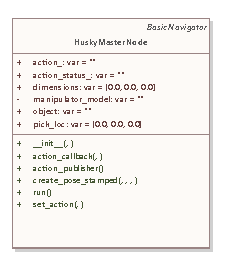
\includegraphics[width = 0.6\textwidth]{Figures/husky_master.pdf}
  \caption{UML Class Diagram of the Husky Master Node. As this is one class and interacts through ROS topics, it appears alone in the class diagram.}
  \label{fig:M:TL:huskyMasterUML}
\end{figure}

Looking at the UML diagram in figure \ref{fig:M:TL:huskyMasterUML}, it can be seen that this class inherits from the class \lstinline{BasicNavigator}. \lstinline{BasicNavigator} is a part of the standard python API towards ROS2 and inheriting from this class gives all the functionality of this class plus additional custom functionality. This means that the interface towards NAV2 is set up from within the \lstinline{BasicNavigator} class. When initiating the HuskyMasterNode class, the constructor \lstinline{__init__(manipulator_model="vx300")} is called. This constructor sets up a subscription to the ROS2 topic \lstinline{/action_status}, and a publisher to the \lstinline{/action} topic. In a similar fashion as with the PickAndPlace class, any data detected on the \lstinline{/action_status} topic, will be stored in the member variable \lstinline{action_status_}. Additionally, the constructor will check if values are given for the parameters "object" (name of object to pick), "dimensions" (dimensions of object to pick $(d[m], w[m], h[m])$ and "pick\_loc" (mobile robot goal pose for object picking, $(x[m], y[m], \theta[rad]))$). If no values are given for these parameters, the constructor will give default values. 

The implementation of this class is shown in greater detail in algorithm \ref{alg:M:HuskyMaster}. It is a relatively basic integration which relies on a predefined sequence of commands to the other subsystems. The place location and home location of the mobile robot is hard coded into the sequence and will have to be changed in the source code if needed.
 


  \begin{algorithm}[htp!]
    \caption{Algorithm describing how the Husky Master node is implemented} \label{alg:M:HuskyMaster}
    \begin{algorithmic}[1] 
            \State $reachedPickLoc \gets$ \textbf{false}
            \State $pickingFinished \gets$ \textbf{false}
            \State $reachedPlaceLoc \gets$ \textbf{false}
            \State $placingFinished \gets$ \textbf{false}
            \State $reachedHome \gets$ \textbf{false}
            \State $timeout \gets 120s$ \Comment{Timeout for while loops}
            
            \State $node \gets HuskyMasterNode$ \Comment{Initiate Husky Master Node}
            \State Wait until NAV 2 is active
            
            \State $Nav2GoalPose \gets pickLoc$ \Comment{Send goal pose to NAV 2}
            
            \While{(\textbf{\textbf{not}} ERROR) \textbf{and} (\textbf{not} $reachedPickLoc$)}
                \If{$nav.isTaskComplete()$}
                    \State $reachedPickLoc \gets$ \textbf{true}
                \EndIf
            \EndWhile
            
            \If{$reachedPickLoc$}
                \State $PickAndPlaceCommandString("pick" + "\;" + object +"\;" + Dimensions")$ 
                \State Send $PickAndPlaceCommandString$ \Comment{Sends on topic "/action"}
            \EndIf
            
            \While{(\textbf{\textbf{not}} ERROR) \textbf{and} (\textbf{not} $pickingFinished$)}
                \If{$nav.actionStatus() == "picking \; finished"$} \Comment{Listens to topic "/action\_status"}
                    \State $pickingFinished \gets$ \textbf{true}
                \EndIf
            \EndWhile
            
            \If{$pickingFinished$}
                \State $Nav2GoalPose \gets placeLoc$ \Comment{Send goal pose to NAV 2}
            \EndIf
            
            \While{(\textbf{\textbf{not}} ERROR) \textbf{and} (\textbf{not} $reachedPlaceLoc$)}
                \If{$nav.isTaskComplete()$}
                    \State $reachedPlaceLoc \gets$ \textbf{true}
                \EndIf
            \EndWhile
            
            \If{$reachedPlaceLoc$}
                \State $PickAndPlaceCommandString("place")$ 
                \State Send $PickAndPlaceCommandString$ \Comment{Sends on topic "/action"}
            \EndIf
            
            \While{(\textbf{\textbf{not}} ERROR) \textbf{and} (\textbf{not} $placingFinished$)}
                \If{$nav.actionStatus() == "picking \; finished"$} \Comment{Listens to topic "/action\_status"}
                    \State $placingFinished \gets$ \textbf{true}
                \EndIf
            \EndWhile
            
            \If{$placingFinished$}
                \State $Nav2GoalPose \gets homeLoc$ \Comment{Send goal pose to NAV 2}
            \EndIf
            
            \While{(\textbf{\textbf{not}} ERROR) \textbf{and} (\textbf{not} $reachedHomeLoc$)}
                \If{$nav.isTaskComplete()$}
                    \State $reachedHomeLoc \gets$ \textbf{true}
                \EndIf
            \EndWhile
            
            \State \textbf{shutdown}
    \end{algorithmic}
 \end{algorithm}

The first five lines of algorithm \ref{alg:M:HuskyMaster} contains declaration of some flags that are set when certain parts of the sequence is fulfilled. The next line contains the declaration of a timeout variable. This variable determines how long each operation (every while-loop in alg. \ref{alg:M:HuskyMaster}) is allowed to run. If for example picking exceeds 120s, it will throw and error and jump out of the while-loop at line 19-23, causing the whole node to stop execution.  Line 7 in algorithm \ref{alg:M:HuskyMaster}, initiates the node as \lstinline{nav}. This is where the constructor is called. When the system has gotten feedback that NAV2 is active (line 8 in alg. \ref{alg:M:HuskyMaster}), it will command NAV2 to navigate towards the goal (line 9 in alg. \ref{alg:M:HuskyMaster}) ad wait for feedback that the goal is reached. When the goal is eventually reached, the node will command the Pick and Place system to pick the object defined in the parameters of this node (line 16 and 17 in alg. \ref{alg:M:HuskyMaster}). The picking operation involves searching for the object as described in section \ref{M:PickAndPlace}. When the node receives a message that picking is finished, it will proceed. The rest of algorithm \ref{alg:M:HuskyMaster} from line 24, is similar to lines 9-23, as it involves sending commands to either NAV2 or Pick and Place and waiting for their response before preforming the next action. When the mobile robot reaches it's home pose again, the node shuts down.

% \begin{figure}[htp]
%   \centering
%   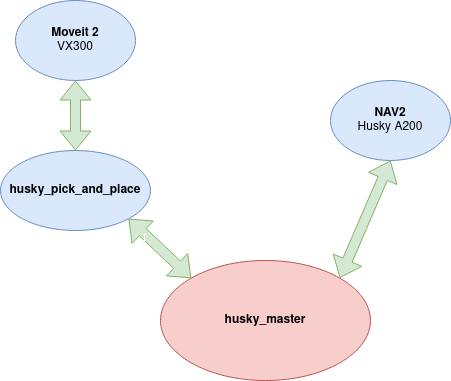
\includegraphics[width = 0.6\textwidth]{Figures/software_overview.drawio.png}
%   \caption{The "husky\_master" node controls the operation by interfacing directly with NAV2 and with Moveit2 through the "husky\_pick\_and\_place" node.}
%   \label{fig:husky_master}
% \end{figure}
